\documentclass{mifcs2}

\usepackage{graphicx}
\graphicspath{{./images/}}
\usepackage{url}

% Xetex

\usepackage{fontspec}
\usepackage{xunicode}
\usepackage{xltxtra}
\setmainfont[Mapping=tex-text]{Times New Roman}

% Xetex end

% Latex

%\usepackage{times}
%\usepackage[utf8x]{inputenc}
%\usepackage{ae,aecompl}

% Latex end


% PDF related options
\usepackage[
  bookmarks=true,
  bookmarksnumbered=true,
  pdftitle={Vokseliais paremtas vizualizavimas},
  pdfauthor={Petras Zdanavičius},
  pdfcreator={XeTeX with hyperref package},
  colorlinks=true,
  linkcolor=black,
  citecolor=black,
  urlcolor=black
]{hyperref}


\title{Vokseliais paremtas vizualizavimas}
\author{Petras Zdanavičius}
\date{Vilnius\\2010}

\def\mentor{lek. Saulius Narkevičius}
\def\doctype{Baigiamasis magistro darbas}
\def\studentstatus{2 kurso, 10 grupės studentas}
\def\signature{parašas}

% Translate
\def\figurename{Pav.}
\def\tablename{Lentelė.}
\def\literature{Literatūros sąrašas}
\renewcommand*{\refname}{\literature}

\begin{document}

% Do not ask about "fancy" and "empty" things...
\maketitle
\thispagestyle{empty}
\tableofcontents
\thispagestyle{empty}
\clearpage
\thispagestyle{fancy}

\section{Anotacija}

Šiame darbe yra pristatomas autoriaus sukurtas vokselių vizualizavimo ir
normavimo įrankis. Įrankis įgalina vartotoją vizualizuoti tūrinius objektus,
tūrinius duomenis pritaikant taip, kad būtų pasiektas kuo galima akiai
malonesnis vaizdas.

Vizualizavimas vyksta realiu laiku. Naudojamas spindulių skleidimo algoritmas.
Derinimui yra pateikti transformavimo bei darbe pasiūlyti globalaus
permatomumo ir apšvietimo sustiprinimo filtrai. Valdymas vyksta realiu laiku
keičiant filtrų parametrus. Didžioji dalis skaičiavimų yra palikti GPU pusei.

Prieš pristatant įrankį, darbe taip pat trumpai apžvelgiami vokseliai ir jų
vizualizavimo idėjos.


\section{Summary}

In this paper author presents tool for voxels' visualization. It lets users to
render volume scene and change how it looks with the help of various options.

It is real-time rendering tool. It uses ray casting. Options consist of
transfer function (controlled in real-time) and author's contribution: global
transparency filter and lighting strengthening filter.

This paper also describes a concept of voxel and other voxels' rendering
methods.


\section{Įvadas}

Su kompiuterinės grafikos vizualizacijomis dirbančios specialiųjų efektų
studijos jau gana seniai pastebėjo, kad kai kuriems efektams (Pavyzdžiui:
rūko, debesų, sprogimų) išgauti poligoninių paviršių vizualizavimas nėra
geriausia išeitis. Ypač jeigu norima pasieki detalų, stambiam planui tinkantį
rezultatą. Tūriniams efektams vizualizuoti dažniausiai pasitelkiamos tūrinių
objektų vizualizavimo technikos, žinomos bendriniu „vokselių vizualizavimo
technologijų“ pavadinimu.

Vokselių vizualizavimas taip pat naudojamas įvairiuose moksliniuose
įrankiuose, kur būtina vaizduoti „neoptimizuotus“ (nepakeistus) tūrinius
objektus (Pavyzdžiui, medicinos tyrimai).

Prieš tai minimi atvejai nėra iš realaus laiko 3D vaizdavimo srities. O
pastarojoje tūrinis vizualizavimas yra ganėtinai apleista sritis. Tą sąlygojo
techninės galimybės. Tačiau dabar aparatūrinė įranga jau įgalina vaizduoti
tūrinius objektus realiu laiku. Būtent šiai sričiai -- tūrinių objektų realaus
laiko vizualizacijai -- šiame darbe yra skiriamas didžiausias dėmesys. Jame
yra pristatomas autoriaus sukurtas realaus laiko vokselių vizualizavimo ir
normavimo įrankis.

Darbo tikslai:

\begin{itemize}
\item Pristatyti vokselių idėją
\item Pristatyti pagrindines tūrinių objektų vaizdavimo koncepcijas
\item Pristatyti sukurtą realaus laiko vokselių vizualizavimo ir
normavimo įrankį
  \begin{itemize}
  \item Apžvelgti transformavimo filtrą
  \item Apžvelgti globalaus permatomumo filtrą
  \item Apžvelgti apšvietimo sustiprinimo filtrą
  \end{itemize}
\end{itemize}

\begin{figure}[b]
\centering
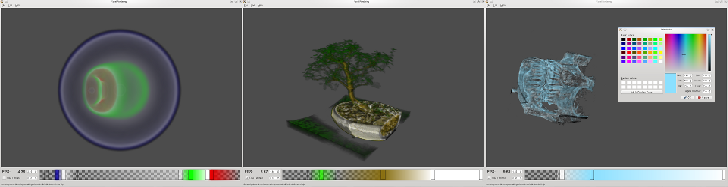
\includegraphics[width=16.5cm]{teaser.png}
\caption{Darbe pristatomas vokselių vizualizavimo ir normavimo įrankis.}
\label{fig:teaser}
\end{figure}


\section{Susiję darbai}
\label{sec:susije_darbai}

Apie spindulių skleidimo idėjos pritaikymą tūriniams objektams vizualizuoti,
naudojant vokselius, kalbama jau 1988 m. Marc Levoy straipsnyje
„\textit{Display Of Surfaces from Volume Data}“ \cite{first}.

Jens Krüger ir Rüdiger Westermann 2003m. publikuotame „\textit{Acceleration
Techniques for GPU-based Volume Rendering}“ \cite{raycast} spindulių skleidimas
įgyvendinamas panaudojant spalvotų vienetinių kubų idėją, kuria aš daugiausiai
ir rėmiausi, kurdamas savo įrankį.

Dabartiniai darbai, naudojantys tūrinį spindulių skleidimą, daugiausia dėmesio
skiria tūrinių scenų su masiniu vokselių skaičiumi vizualizavimui. Tai Cyril
Crassin ir kiti autoriai su savo veikalais „\textit{Interactive GigaVoxels}“
\cite{gig2008} ir „\textit{GigaVoxels : Ray-Guided Streaming for Efficient and
Detailed Voxel Rendering}“ \cite{gig2009}. Juose pristatomas tūrinio skleidimo
algoritmas. Tačiau dėl to, kad jie bando dirbti su dideliu kiekiu duomenų --
jie privalo daryti tam tikras prielaidas (pvz.: kad dauguma objektų visiškai
nepermatomi).

Enrico Gobbetti ir kiti autoriai taip pat panaudojo spindulių skleidimą
masiniam vokselių vizualizavimui darbe „\textit{A single-pass GPU ray casting
framework for interactive out-of-core rendering of massive volumetric
datasets}“ \cite{other}. Kitaip nei prieš tai aptartų darbų autoriai, šie
visiškai atsisako dalinio permatomumo, tačiau dėl to leidžia sau naudotis
agresyvia vokselių blokelių atmetimo technika.


\section{Plačiau apie vokselius}

\subsection{Vokselis}

Pradėkime nuo vokselio apibrėžimo:

{\bf Vokselis} -- tūrinis elementas, reprezentuojantis patį mažiausią galimą
diskretizuotos trimatės erdvės elementą.

Pakankamai paprastas apibrėžimas, bet galimi ir kitokie jo variantai:

Sukapokime stačiakampio gretasienio (gali būti ir kubas) aprėpiamą erdvę į
$LxNxM$ elementus. Visi tie maži stačiakampiukai gretasieniai ir bus
{\bf vokseliai}.

\begin{figure}
\centering
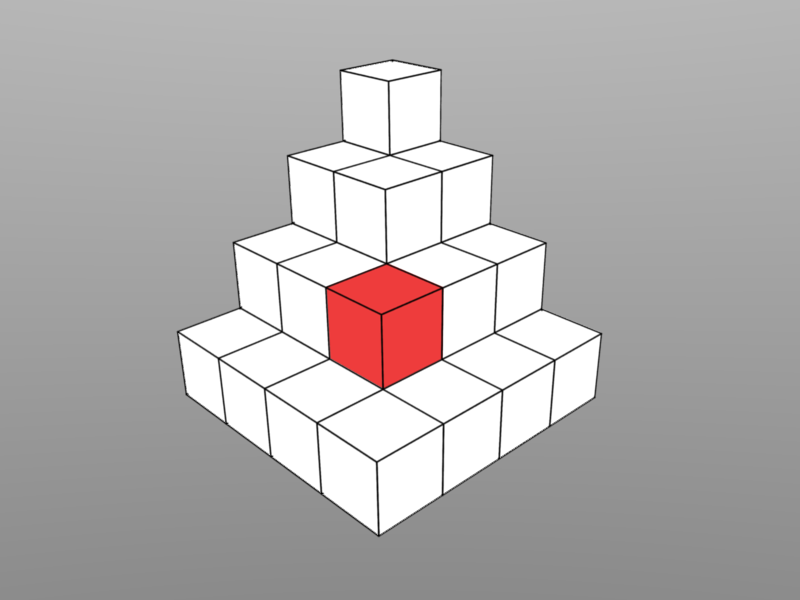
\includegraphics[height=6cm]{voxels.png}
\caption{Vokseliai (visi kubai) ir vokselis (raudonas kubas).}
\label{fig:voxels}
\end{figure}

Vokselis yra dvimačio objekto -- fragmento (su tam tikromis išlygomis galima
prilyginti pikseliui) praplėtimas trimatėje erdvėje. Kaip ir fragmento, taip
ir vokselio pagrindinė savybė yra jo pozicija. Tik vokseliai dar turi ir $Z$
koordinatę. Visos kitos vokselio savyje nešamos informacijos kiekis priklauso
nuo panaudojimo reikmių. Kaip ir fragmentų atveju, populiariausios yra $RGB$
ir $RGBA$ ($R$ -- \emph{red}, raudona; $G$ -- \emph{green}, žalia; $B$ --
\emph{blue}, mėlyna; $A$ -- \emph{alpha}, permatomumo) duomenų komponentės.
Kitaip nei fragmente, taip pat gana dažnai vokselis turi savo normalės
duomenis -- vis dėlto perlipama į trimatę erdvę.

To pačio vokselio interpretavimas, vėlgi, gana stipriai priklauso nuo tūrinui
vizualizavimui juos panaudojančios aplikacijos poreikių. Pavyzdžiui: Galima
laikyti, kad vokselių reikšmės yra „gry-nos“ tik jų centruose -- visur kitur
tūrio reikšmės yra interpoliuojamos tarp gretimų centrų reikšmių. Taip pat
galima laikyti, kad tūrinio objekto erdvės, kurią gaubia vokselis, įvairios
reikšmės (Pavyz-džiui $RGBA$) yra vienodos ir jas apibrėžia tas duotasis
vokselis.

\subsection{Panaudojimo sritys}

Visų pirma reiktų paminėti mokslinius įvairių sričių tyrimus. Medicina,
archeologija, biologija -- turbūt būtų plačiausiai tūrinį vizualizavimą
naudojančios mokslo sritys. Tūrinis vizualizavimas (o tuo pačiu ir vokselių
idėjos) jose dažniausiai naudojamos, vaizduojant įvairius duomenis.
Pavyzdžiui: kompiuterinės tomografijos, magnetinio rezonanso, ultragarso.
Moksle vokseliai naudojami, nes neretai ten būtina žinoti (ir matyti) visą
tūrinį objektą ir jį sudarančius vokselius -- o tam vien trimačių paviršių
neužtenka.

Žinoma, vien „rimtaisiais“ mokslais vizualizavimas neužsibaigia. Visa
volumetrikos idėja taip pat yra panaudojama tiesiog gražiems (priklauso nuo
skonio) vaizdams generuoti. Daugiausia vie-tos po saule vokseliai yra
išsikovoję vaizdo medžiagos specialiųjų efektų srityje.

Tuo tarpu viena iš plačiausiai trimatę grafiką naudojančių sričių --
kompiuteriniai žaidimai -- tūrinį vizualizavimą yra primiršę ir paprastai
išsiverčia tik su paviršių (poligonų) vizualizavimu. Bet populiarėjant
kompiuteriniams žaidimams ir vis gerėjant aparatūrinei įrangai, didės vis
kokybiškesnių ir kokybiškesnių realaus laiko kompiuterinės grafikos vaizdinių
poreikis. Tada žaidimų kūrėjai susidurs su tomis pačiomis problemomis, su
kuriomis jau susidūrė specialiųjų efektų studijos -- kai kurie efektai tiesiog
„nesižiūri“, naudojant vien tik paviršius. Tikėtina, kad tuo metu atsiras
hibridiniai (tiek vokselius, tiek poligonus) panaudojantys žaidimų varikliukai
(Industrijoje jau sklando kalbos, kad tokie varikliukai yra kuriami duotuoju
momentu).

\subsection{Tūrinių ir poligoninių objektų palyginimas}

Gali susidaryti įspūdis, kad vokseliai realaus laiko kompiuterinėje grafikoje
tiesiogiai konkuruoja su poligonais. Gal taip ir buvo praeityje, bet dabar to
nėra, o ir ateityje mažai tikėtina, kad tas pasikartos -- greičiau jau išvysime
šių dviejų (ir kelių kitų) vizualizavimo koncepcijų susiliejimą ir bendrą
naudojimą, nei kad kuri nors iš jų dominuos, o kitos liks užmarštyje.

\subsubsection{Tūriniai objektai}

\begin{figure}[!ht]
\centering
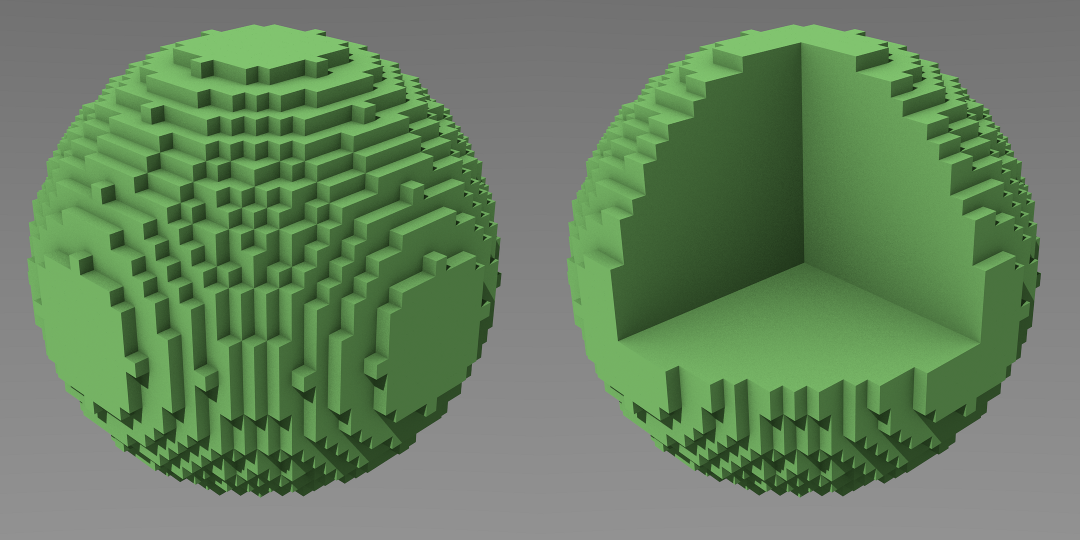
\includegraphics[width=16.5cm]{voxel_sphere.png}
\caption{Sfera, sudaryta iš vokselių. Pastaba: iliustraciniais tikslais
pasirinktas mažas detalumo lygmuo ir vizualizuojant nepritaikytos jokios
kampuotumą išlyginančios metodikos.}
\label{fig:voxel_sphere}
\end{figure}

Pliusai:

\begin{itemize}
\item Tūris
\item Detalumas
\item Pusiau permatomų objektų tikroviškumas
\item Paprastesnė duomenų struktūra
\end{itemize}

Minusai:

\begin{itemize}
\item Reikalauja daug atminties
\item Sudėtingas deformuojančio (Pavyzdžiui: kaulinė) animacijos įgyvendinimas
\item Aparatūrinės įrangos palaikymo nebuvimas
\item Mažas tūrinių objektų kūrimo įrankių pasirinkimas
\end{itemize}

\subsubsection{Poligonai objektai}

\begin{figure}[!ht]
\centering
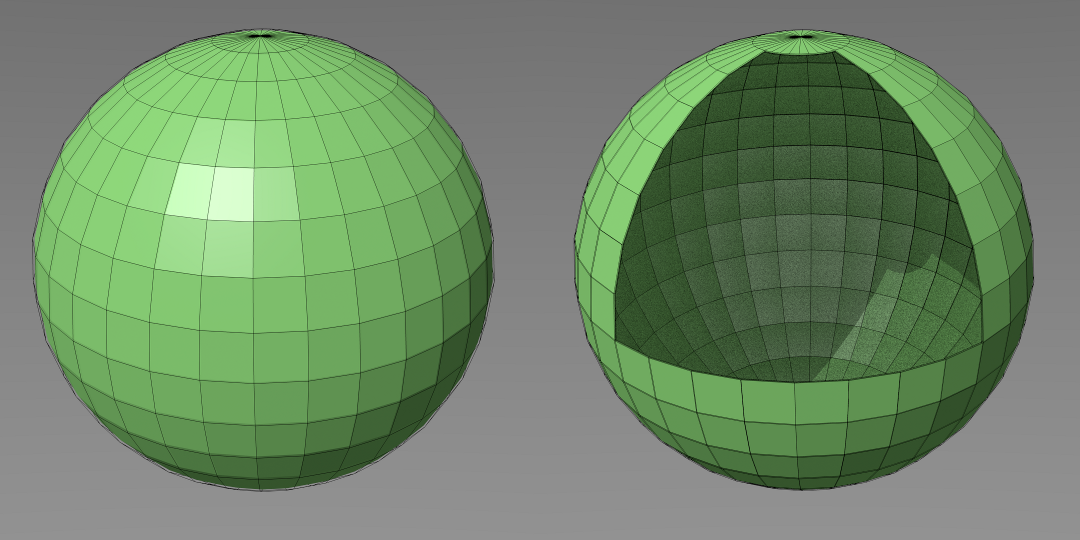
\includegraphics[width=16.5cm]{poly_sphere.png}
\caption{Sfera, iš poligonų. Atkreipkite dėmesį, kad ji tuščiavidurė.}
\label{fig:poly_sphere}
\end{figure}

Pliusai:

\begin{itemize}
\item Reikalauja mažiau atminties
\item Ganėtinai gerai prisitaiko prie deformuojančios animacijos
\item Gausybė kūrimo įrankių
\item Aparatūrinės įrangos palaikymas
\end{itemize}

Minusai:

\begin{itemize}
\item Prastokai susidoroja su pusiau permatomų objektų perteikimu
\item Sudėtingesnė duomenų struktūra
\item Tuščiaviduriai objektai
\end{itemize}

Tai nėra labai nuodugnus palyginimas, tačiau iš jo gana akivaizdu, kad
kiekviena koncepcija turi savo panaudojimo situacijas.

Pavyzdžiui: reikia vizualizuoti žmogaus kūną, kuris atliks įvairius judesius.
Ypatybės: nepermatomas objektas; deformuojančios animacijos. Pasirinkimas:
poligonai.

Reikia pavaizduoti dūmus. Ypatybės: pusiau permatomas tūrinis objektas;
dalelyčių animacija. Pasirinkimas: vokseliai.

Reikia pavaizduoti siena. Pasirinkimas: poligonai. Tą sieną bus galima
naikinti realiu laiku (tarkim betono siena, kurią galima išsprogdinti
dalimis). Tuomet pasirinkimas: vokseliai.

Akivaizdu, kad niekas netrukdo integruoti šias abi koncepcijas viena į kitą.
Pavyzdžiui: poligoninis nepermatomas žmogus formuoja vokselinę ledo skulptūrą.
Jis ne tik keičia skulptūros formą, bet ir pridaro joje daug skylių.


\section{Kompiuteriniai žaidimai ir vokseliai}

Realaus laiko kompiuterinės grafikos beveik visos inovacijos ir novatoriškos
idėjos atkeliauja per kompiuterinių žaidimų industriją. Ne išimtis ir
vokselizavimo idėja. Čia pateikiama trumpa ir nepilna kompiuterinių žaidimų
istorija, išskirtinį dėmesį rodant vokselizavimo idėjas panaudojusiems
žaidimams.

\subsection{Istorija}

\begin{list}
{
}
{
  \setlength\leftmargin{2.43cm}
  \setlength\labelwidth{3cm}
  \setlength\labelsep{1cm}
}

\item[1986 m.] {\bf Starglider} (Pav. \ref{fig:game_starglider}). Labai
primityvūs trimatę grafiką imituojantys tinkleliai.

\begin{figure}[!ht]
\centering
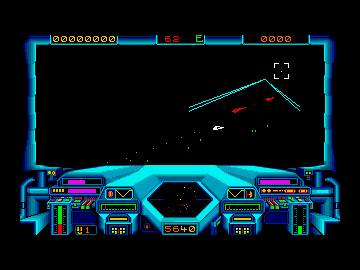
\includegraphics[height=5.0cm]{game_starglider.png}
\caption{Starglider. \emph{MobyGames}\copyright}
\label{fig:game_starglider}
\end{figure}

\item[1988 m.] {\bf F-19 Stealth Fighter}. Tinklelio paviršius užpildomas apvalkalu
ir taip pristatomi poligonai.

\item[1992 m.] {\bf Wolfenstein}. Pristatomos tekstūros. Dėl greičio
atsisakoma tikrojo 3D ir jam imituoti panaudojama spindulių skleidimo
(\emph{Ray Casting}) technologija.

\item[1993 m.] {\bf Comanche} (Pav. \ref{fig:game_comanche}). Panaudojami
vokseliai. Žaidimas pasižymi tiems lai-kams ypač detale aplinka.

\begin{figure}[!ht]
\centering
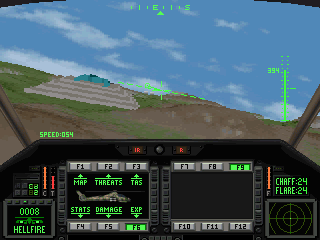
\includegraphics[height=5.0cm]{game_comanche.png}
\caption{Comanche. \emph{NovaLogic}\copyright}
\label{fig:game_comanche}
\end{figure}

\item[1993 m.] {\bf Strike Commander}. Žaidimas, sujungęs tekstūras su
poligonais. Marges-nė ir netokia kampuota kaip Comanche išvaizda, bet iki
pastarojo detalumo lygmens Strike Commander buvo toloka.

\item[1996 m.] {\bf Quake} (Pav. \ref{fig:game_quake}). Prie poligonų ir
tekstūrų pridedami šviesos žemėlapiai (\emph{lightmaps}). Tai leido pasiekti
tuo metu įspūdinga detalumo lygmenį.

\begin{figure}[!ht]
\centering
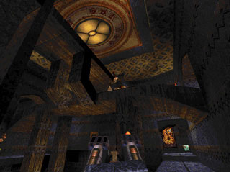
\includegraphics[height=5.0cm]{game_quake.png}
\caption{Quake. \emph{id Software}\copyright}
\label{fig:game_quake}
\end{figure}

\item[1997 m.] {\bf Quake II}. Kompiuterinėje įrangoje įsitvirtina trimatės
grafikos spartintuvai, skirti poligonų vaizdavimui. Šis žaidimas tuo metu bene
geriausiai demonstravo tų įrenginių savybes.

\item[1998 m.] {\bf Delta Force} (Pav. \ref{fig:game_deltaforce}). Ypač
didelėms atviroms aplinkoms buvo panaudotos vokselių technologijos. Žaidimo
variklis buvo pajėgus demonstruoti „begalinius“ atstumus, „begaliniu“
apžvalgos kampu, tačiau vokseliais paremtos technologijos neišnaudojo grafikos
spartintuvų.

\begin{figure}[!ht]
\centering
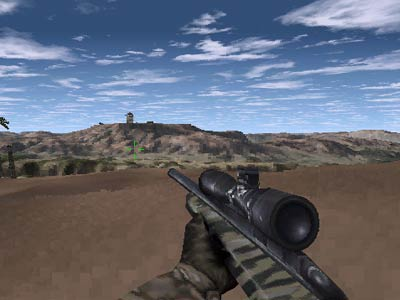
\includegraphics[height=5.0cm]{game_deltaforce.png}
\caption{Delta Force. \emph{NovaLogic}\copyright}
\label{fig:game_deltaforce}
\end{figure}

\item[1999 m.] {\bf Outcast} (Pav. \ref{fig:game_outcast}). Paskutinis, prieš
pertrauką, nusisekęs trimatis žaidimas, naudojęs vokselius.

\begin{figure}[!ht]
\centering
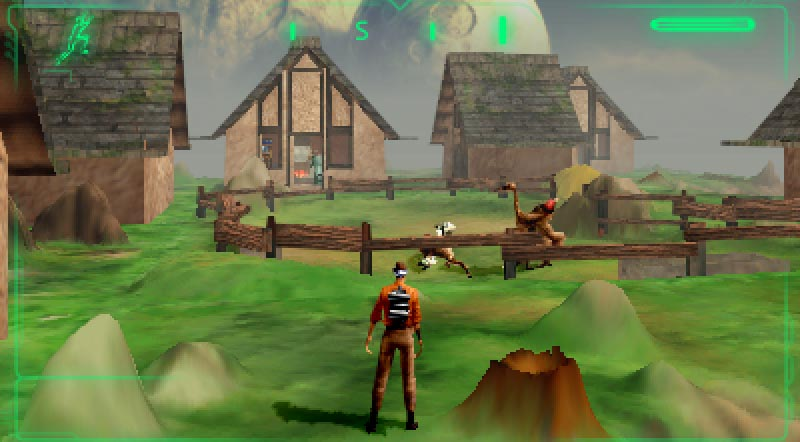
\includegraphics[height=5.0cm]{game_outcast.png}
\caption{Outcast. \emph{Appeal}\copyright}
\label{fig:game_outcast}
\end{figure}

\item[...] Daug, daug tik poligonus naudojančių žaidimų ir žaidimų varikliukų.

\item[2008 m.] \emph{Id Software} Siggraph konferencijoje pristatė vokselių
vizualizavimo technologiją, kuri, tikėtina, bus panaudota būsimajame \emph{Id
Tech 6} varikliuke.

\item[2009 m.] \emph{CryTek} CEDEC konferencijoje paskelbė, kad jų būsimas
varikliukas \emph{Cry-Engine 3} turės galimybę vizualizuoti vokselius.


\end{list}

\subsection{Komentaras}

Visa ši chronologinė tvarka parodo, kad vokseliai kokį dešimtmetį buvo
nenaudojami žaidimų industrijoje. Realaus laiko kompiuterinės grafikos aušroje
buvo bandomos įvairios technologijos ir įvairūs vaizdų generavimo būdai.
Tačiau galiausiai buvo nusistovėta ties poligoniniu vaizdavimo modeliu.

Pagrindinis lūžis įvyko 1996 m. $\sim$ 1997 m. Būtent tada paaiškėjo, kad
trimatės grafikos spartintuvai niekur nedings ir taps neatsiejama asmeninių
kompiuterių ir žaidimų konsolių dalimi.

Vaizdo plokščių atsiradimas stipriai pastūmėjo tiek realaus laiko, tiek visos
kompiuterinės grafi-kos vystymąsi. Tačiau tuo pačiu jų atsiradimas nubrėžė gana
aiškias ribas. Pirmųjų spartintuvų funkcionalumas apsiribojo ties gebėjimu
atvaizduoti daug („daug“ kito nuo laikmečio) trikampių. Taigi, poligoniniai
(trianguliuoti) paviršiai įgijo gana didelį aparatūrinį pranašumą prieš visas
kitas technologijas.

Tačiau viskas vystosi ir keičiasi. Dabartiniai GPU (\emph{Graphics Processing
Unit}) sugeba daugiau nei vien vaizduoti trikampius. Vaizdo plokštės,
nepaisant pavadinimo, patapo bendrinės paskirties, didelį kiekį
mikroprocesorių turinčiais įrenginiais, kurių veikseną galima keisti, nes GPU
be visa ko dar patapo programuojamais -- dabartiniai įrenginiai leidžia
dinamiškai keisti jų pačių veikseną.

Tuo pačiu prasiplėtė ir vaizdavimo ribos, taip atverdamos kelią naujų
vizualizavimo būdų atsiradimui ir senųjų (kartu su vokseliais) grįžimui.
Programuojamos sąsajos leidžia kūrėjams stipriai pakeisti GPU veikseną taip,
kad anos sugeba greitai ir gerai vizualizuoti net tik poligonus.


\section{Vokselių vizualizavimas}

Galima būtų išskirti dvi vokselių vizualizavimo koncepcijas: tiesiogines ir
netiesiogines.

Netiesioginės – tai tūrinio objekto vertimas į paviršių ir pastarojo
vizualizavimas. Tiesioginės tuo tarpu stengiasi išvengti konvertavimo žingsnio
ir viską atlikti, išlaikant visus tūrinius duomenis.

\subsection{Netiesioginis}

Nepaisant šiandieninių techninių galimybių ir naujovių, poligonai vis dar
gana stipriai dominuoja realaus laiko kompiuterinėje grafikoje (ir
nepanašu, kad ketina užleisti lyderės poziciją). Taigi, vienas iš būdų
atlikti tūrinio objekto vizualizavimą yra pastarojo vertimas į paviršių
ir to paviršiaus vaizdavimas. Tūrinis objektas dalyvauja tik
konvertavimo žingsnyje -- visa kita yra darbas su tų tūrių poligonine
imitacija.

Netiesioginio vizualizavimo pliusai:
\begin{itemize}
\item Poligonai -- vis dar pats populiariausias būdas vizualizuoti realiame laike
\item Pats konvertavimas yra vienkartinis procesas
\end{itemize}

Minusai:
\begin{itemize}
\item Tūrinį objektą konvertavus į paviršių, prarandamas pats tūris
\item Netinka pusiau permatomiems objektams
\item
  Konvertuoti gali tekti ir ne vieną kart -- jeigu tūrinis objektas
  interaktyviai keičiasi pačio vizualizavimo metu
\end{itemize}

\subsection{Žygiuojančių kubų algoritmas}

Žygiuojančių kubų algoritmas (\emph{Marching Cubes}) \cite{bib:marching-cubes}
-- vienas iš bazinių tūrinių duomenų netiesioginių vizualizavimo algoritmų.
Pagrindinė idėja yra imti ir padalinti erdvę į mažus kubelius. Šitas
padalijimas nebūtinai turi sutapti su erdvėje esančiais vokseliais – nei jų
dydžiu, nei jų orientacija. Netgi geriau jeigu nesutaps. Tada keliauti per
kiekvieną iš kubų ir žiūrėti kiek, kurios ir kaip kubų kraštinės kertasi su
duotais vokseliais. Galima atskirti trimatės gardelės viršūnes -- tas, kurios
yra objekto viduje ir tas, kurios yra išorėje. Pagal surinktus susikirtimų
duomenis paskaičiuojamas vokselius aproksimuojantis paviršius (Pav.
\ref{fig:marchingcubes_steps}). Algoritmas kreipia dėmesį tik į tas kraštines,
kurios turi skirtingos kategorijoms priklausančias viršūnes.

\begin{figure}[b]
\centering
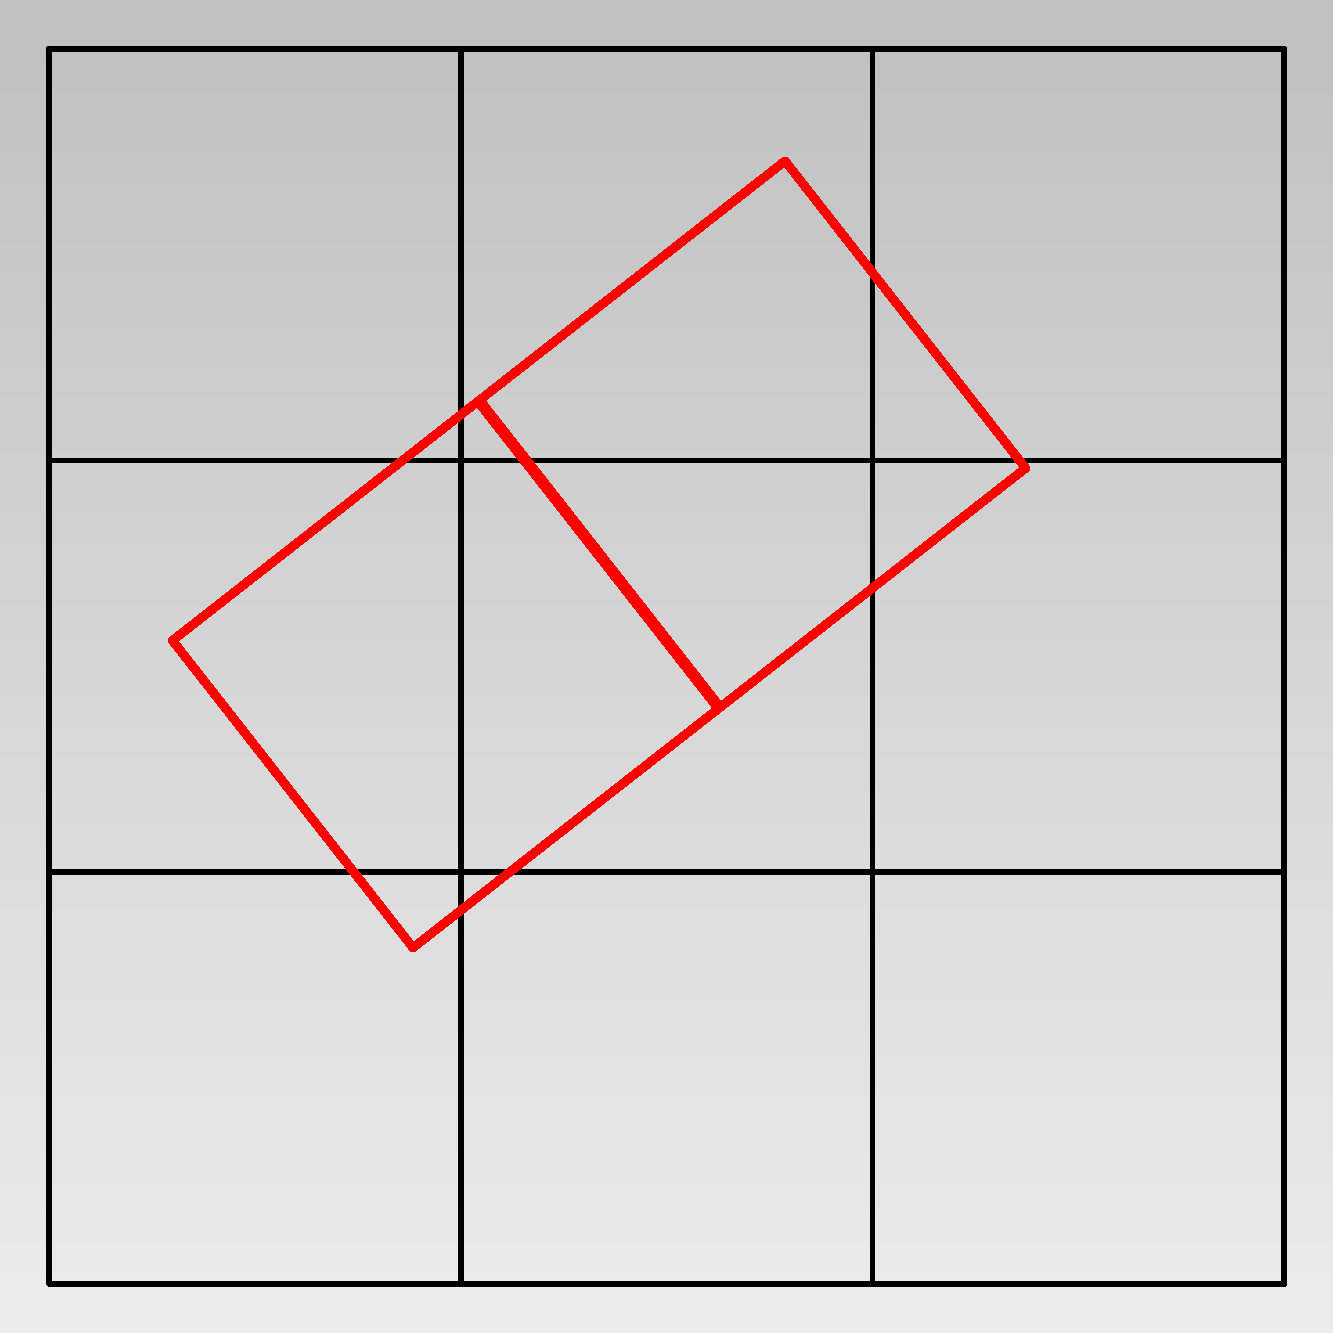
\includegraphics[height=4.5cm]{marching_cubes_step1.pdf}
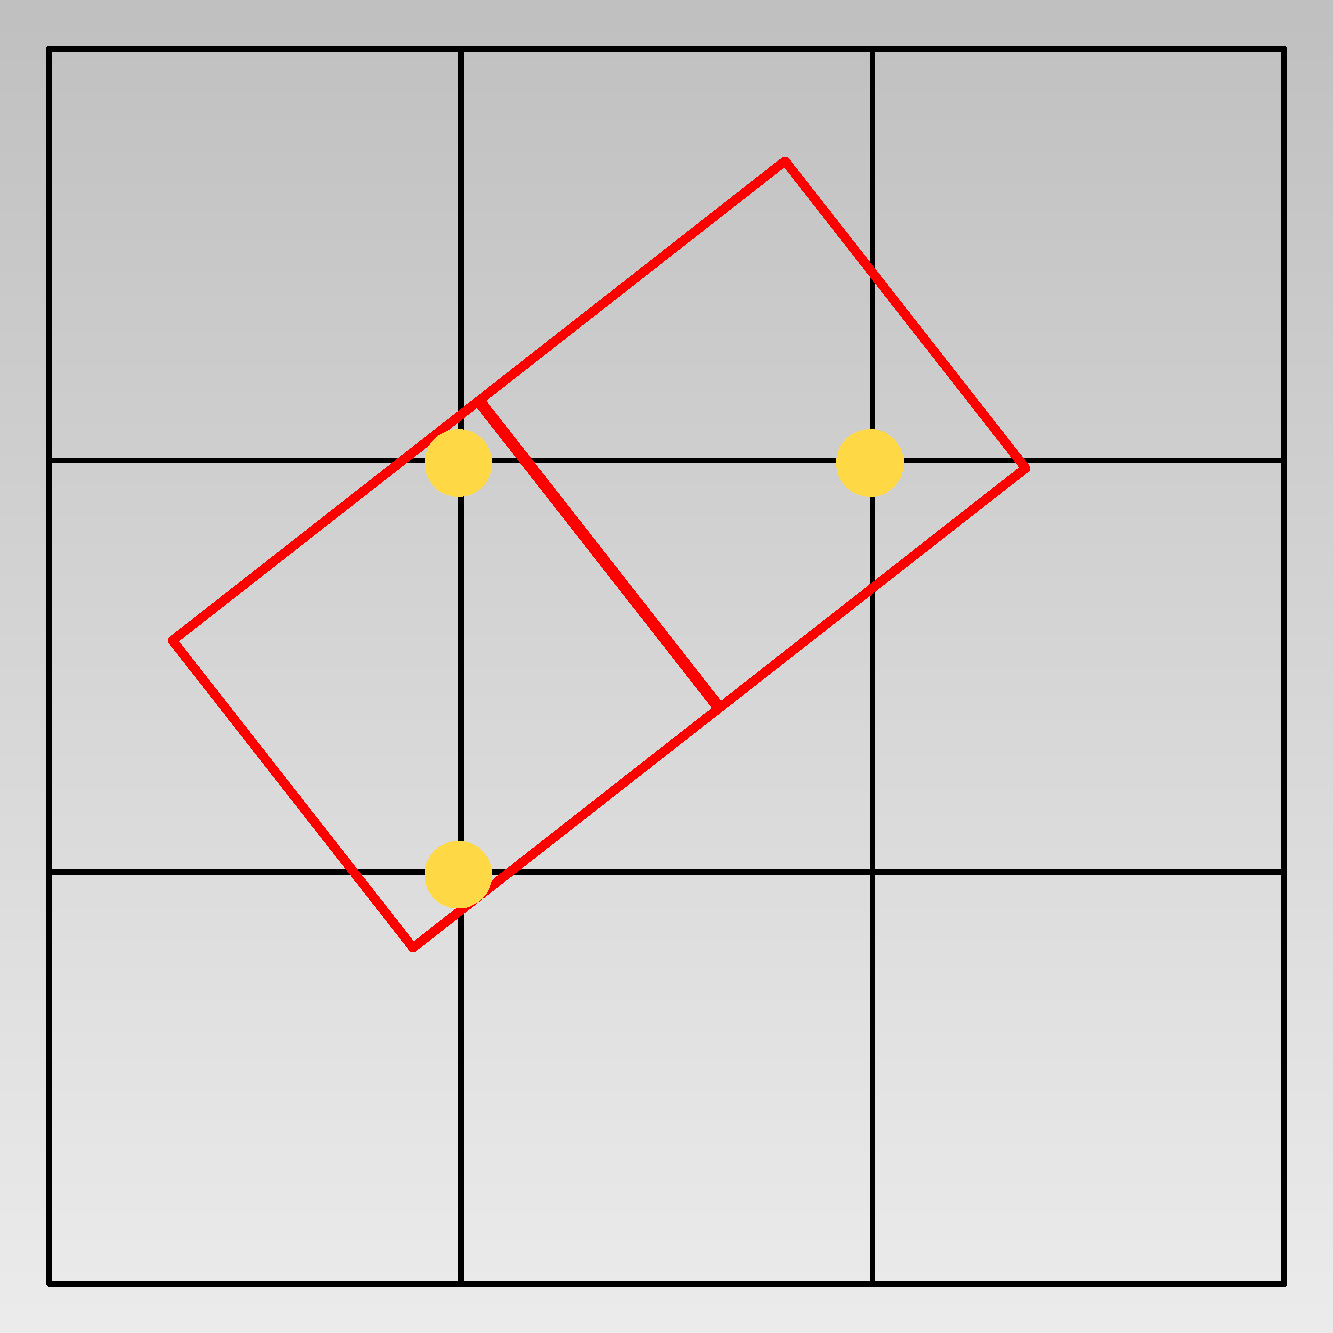
\includegraphics[height=4.5cm]{marching_cubes_step2.pdf}
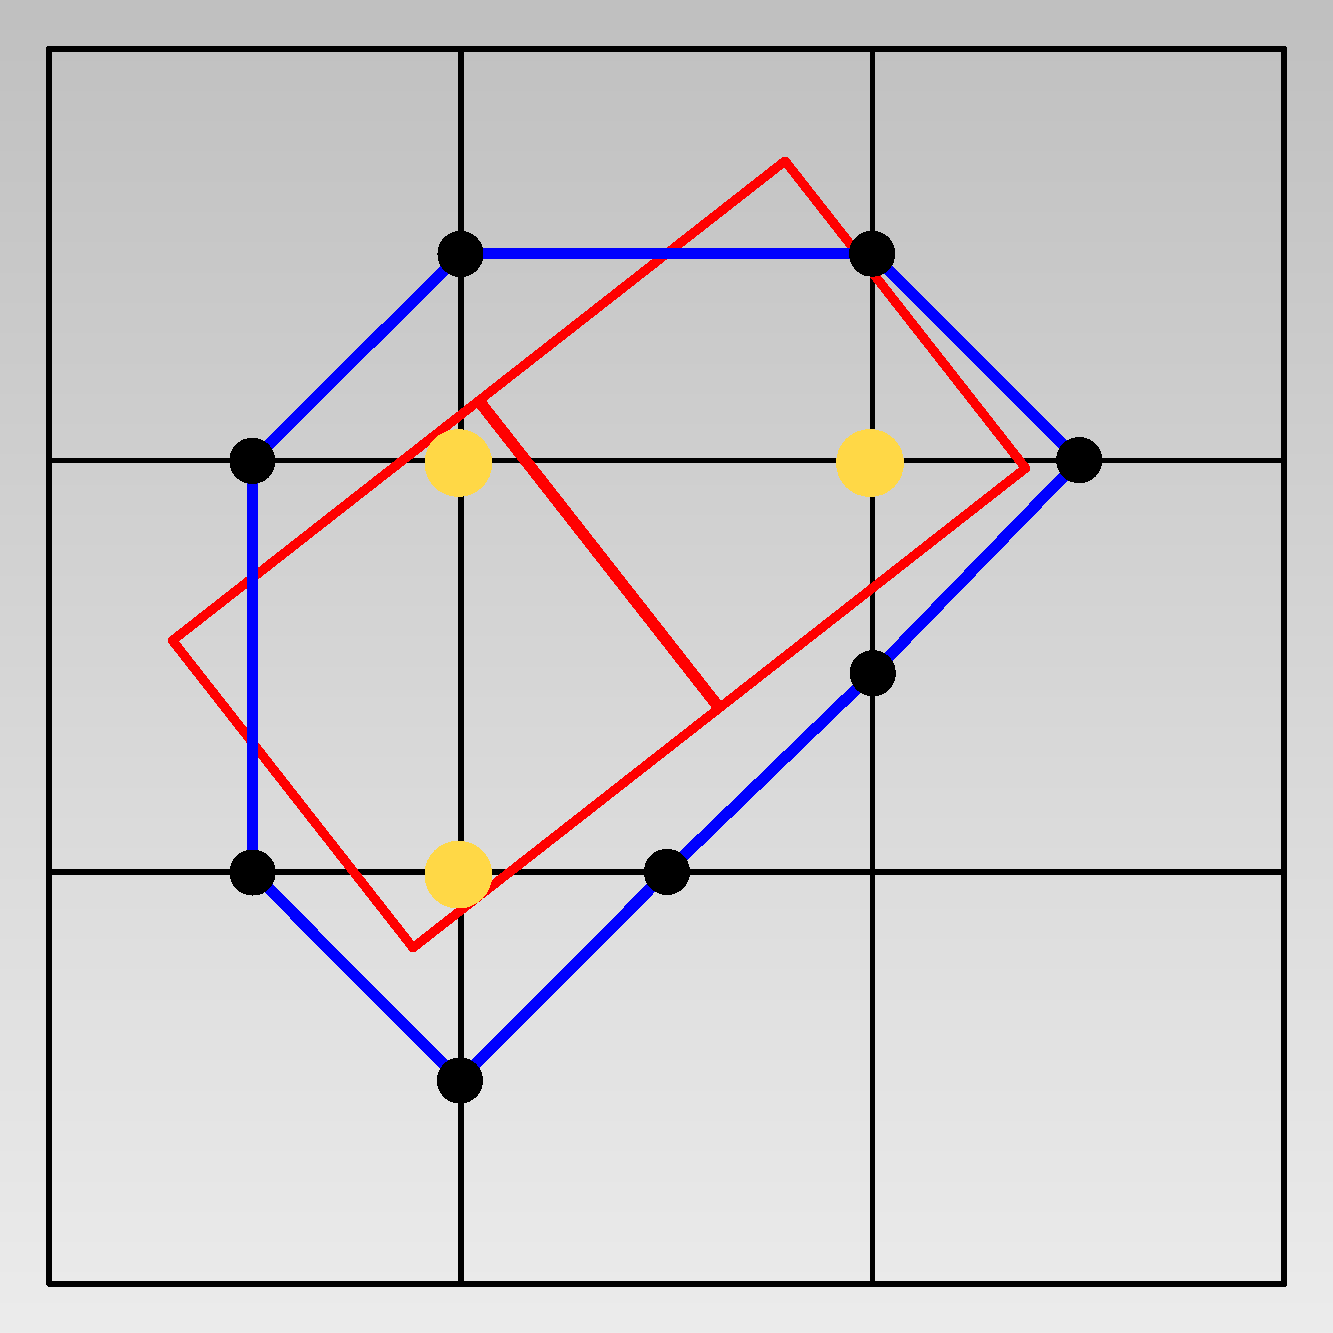
\includegraphics[height=4.5cm]{marching_cubes_step3.pdf}
\caption{2D pjūviai: Erdvės padalijimo (juoda) ir vokselių (raudona); Tūrinio
objekto viduje, esančios gardelės viršūnės (oranžinė); Suformuotas paviršius
(mėlyna)}
\label{fig:marchingcubes_steps}
\end{figure}

\subsection{Panaudojant 2D tekstūras}

Tai tiesioginis vizualizavimo būdas. Erdvė yra sukapojama pjūviais
(lygmenimis, diskais) atsisukusiais priekiu į kamerą (Pav.
\ref{fig:2d_tex_layers}). Tada, yra keliaujama nuo galo į priekį sumuojant
spalvines ir permatomumo reikšmes. Galima įvesti šiokį tokį poligonizavimą ir
pjūvius vaizduoti kaip poligo-nus, o jų spalvines ({\em RGBA}) reikšmes kaip
tekstūras (Pav. \ref{fig:2d_tex_camera}). Pagrindinė bėda ta, kad kiekvieną
kartą, pasikeitus apžvalgos kampui, reikia generuoti tiek poligonus, tiek
pačias tekstūras.

\begin{figure}[!ht]
\centering
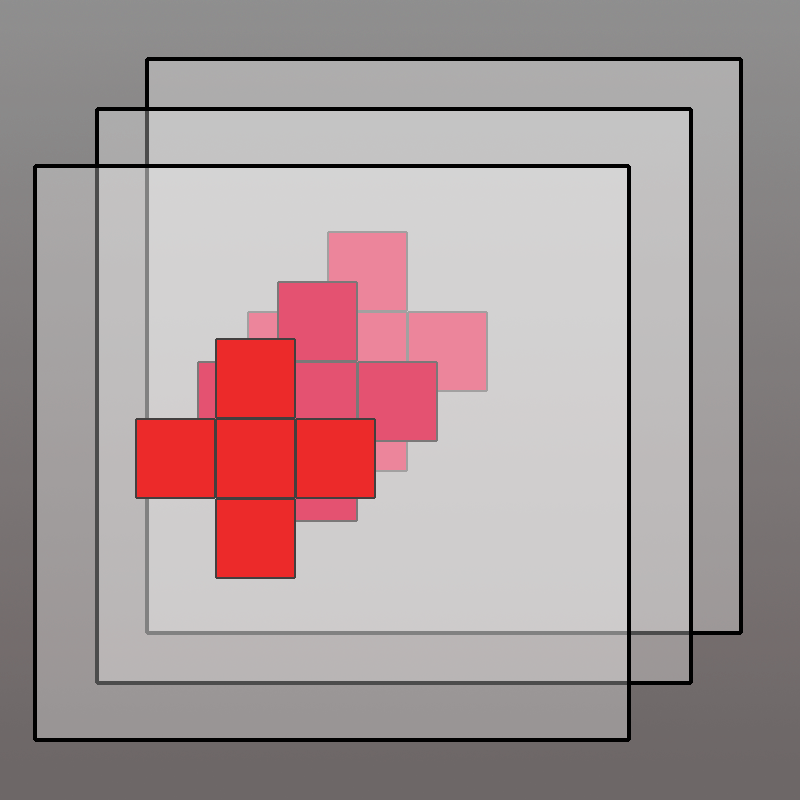
\includegraphics[height=6.5cm]{2d_tex_layers.png}
\caption{Sumuojant pjūvių reikšmes, gaunamas galutinis vaizdas}
\label{fig:2d_tex_layers}
\end{figure}

\begin{figure}[!ht]
\centering
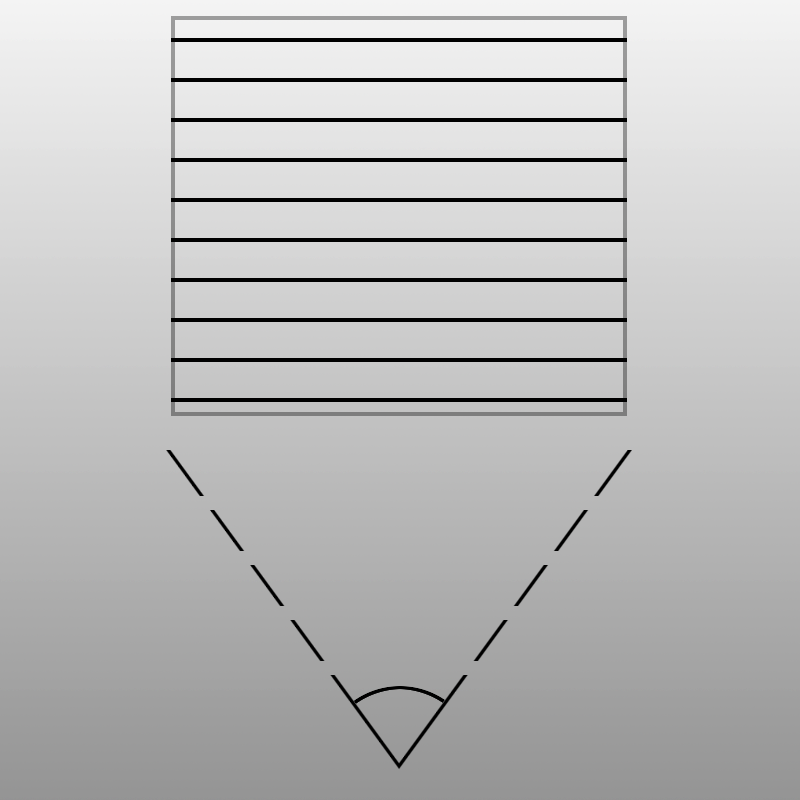
\includegraphics[height=5.5cm]{2d_tex_90.png}
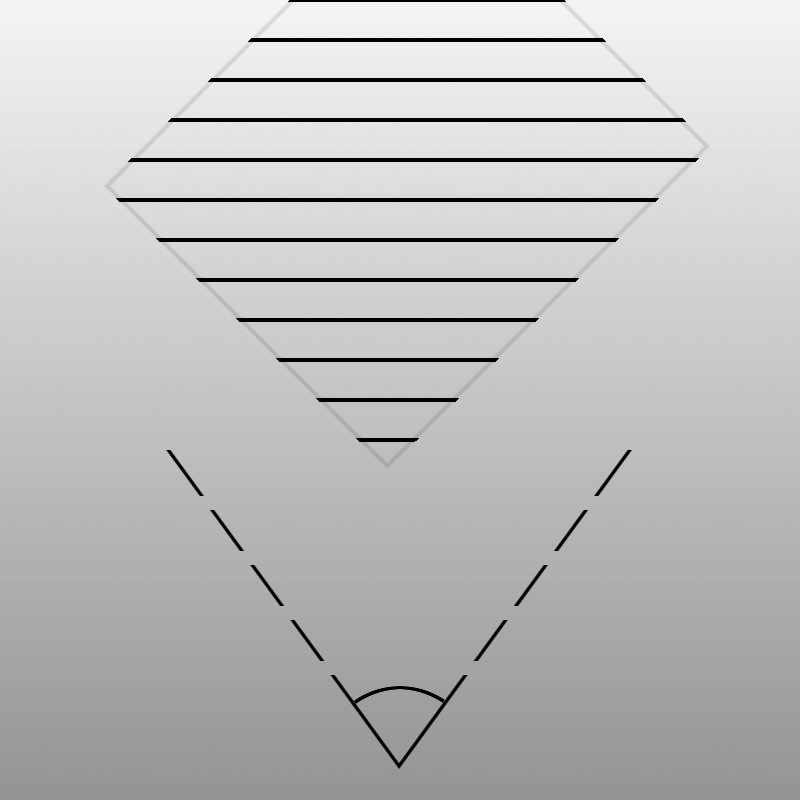
\includegraphics[height=5.5cm]{2d_tex_45.png}
\caption{Kiekvieną kartą keičiantis apžvalgos kampui, būtina perskaičiuoti
tiek pjūvius, tiek tekstūras}
\label{fig:2d_tex_camera}
\end{figure}

\clearpage

\subsection{Panaudojant 3D tekstūras}

Tai tiesioginis vizualizavimo būdas. Labai primena būdą, naudojant 2D
tekstūras. Tik šiuo atve-ju visi duomenys yra saugomi 3D tekstūroje.
Tada generuojant pjūvius, nebereikia pergeneruoti tekstūros -- užtenka tiesiog
teisingai parinkti pjūvių viršūnių tekstūrų koordinates. Kadangi nereikia
generuoti tekstūrų, tai ir įvairius tarpinius duomenų nuskaitymo žingsnius
(tokius kaip interpoliacija) galima palikti aparatūrinei įrangai ir/ar
grafinėms bibliotekoms.

\subsection{Tūrinis spindulių skleidimas}

Pagrindinė tūrinis spindulių skleidimo  (\emph{Ray Casting}. Pav.
\ref{fig:ray_casting}) idėja šiek tiek primena spindulių trasavimo (\emph{Ray
Tracing}) algoritmą. Spindulys yra skleidžiamas iš kameros pozicijos į sceną,
susidedančią iš tūrinių objektų. Spindulio kelionės metu, kaupiama fragmento
spalvų ir permatomumo reikšmės. Tačiau, kitaip nei spindulių trasavime,
procedūra nėra rekursyvi.

\begin{figure}[!ht]
\centering
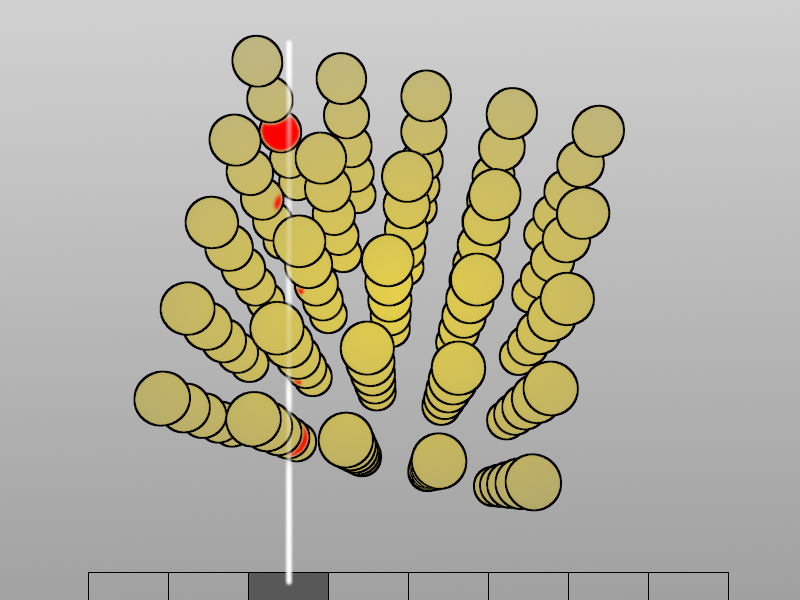
\includegraphics[height=8.0cm]{ray_casting}
\caption{Tūrinis spindulių skleidimas.}
\label{fig:ray_casting}
\end{figure}


\section{Vokselių vizualizavimo ir normavimo įrankis}

Šiame skyriuje pristatomas šio darbo autoriaus sukurtas vokselių vizualizavimo
ir normavimo įrankis (Pav. \ref{fig:tool}), kuris remiasi tūriniu spindulių
skleidimu. Įrankis taip pat įgalina pasinaudoti transformavimo filtru ir šiame
darbe pasiūlytais globalaus permatomumo bei apšvietimo sustiprinimo filtrais.
Įrankis didžiąją dalį skaičiavimų atlieka GPU, o ne CPU.

\begin{figure}[!ht]
\centering
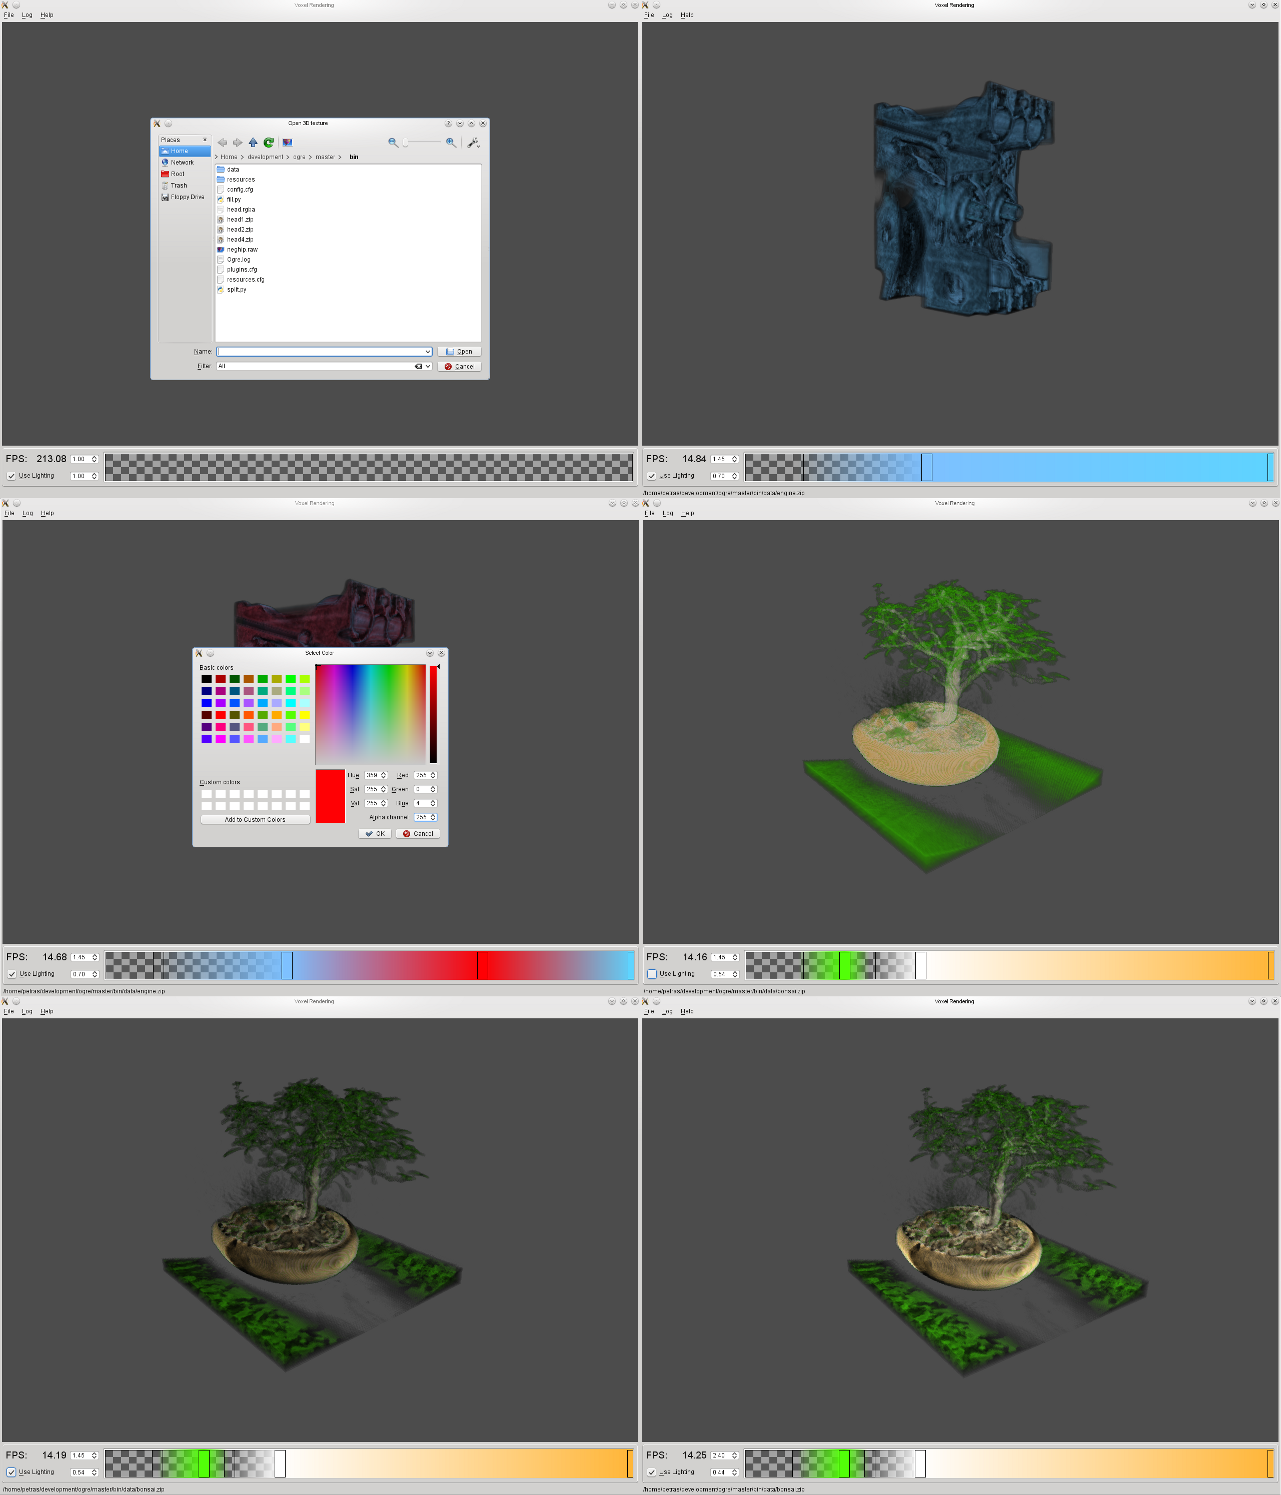
\includegraphics[height=15cm]{tool.png}
\caption{Vokselių vizualizavimo ir normavimo įrankis}
\label{fig:tool}
\end{figure}


Priešingai nei daugelis dabartinių vokselius tyrinėjančių autorių darbų, darbe
pristatomu įrankiu stengtasi atskleisti truputį kitą vizualizavimo pusę --
vietoje bandymo pavaizduoti kuo galima dides-nį kiekį vokselių, įrankis
įgalina pavaizduoti gana ribotą kiekį vokselių. Bet masiškumo praradimą jis
kompensuoja vartotojo sąsajos ir parametrų keitimo lankstumu, bei pačio gauto
vaizdo kokybe.

\subsection{Naudota duomenų struktūra}

Šiuolaikinėje realaus laiko grafikai vizualizuoti šiais laikais beveik visada
yra pasitelkiama vaizdo spartintuvų (\emph{Graphics Processing Unit} -- toliau
GPU) pagalba. Neišmintis ir šis darbas. Vienintelis duomenų pasiekimo būdas,
šiuo metu palaikomas GPU, yra tekstūros, į kurias galima žvelgti kaip į
N-mačius masyvus. Šiame darbe pristatomame įrankyje visi tūriniai duomenys yra
saugomi trimatėje tekstūroje, susidedančioje iš RGBA elementų.

\begin{itemize}

\item
\emph{A} komponentė naudojama kaip vokselio permatomumo reikšmė.

\item
\emph{RGB} komponentės naudojamos saugoti gradientą (tarsi „3d normalė“). Gradientas
yra reikalingas apšveitimui.

\end{itemize}

\subsection{Spalvų kubai}

Kaip jau minėta, esminė įrankyje įgyvendinto spindulių sklaidos algoritmo
idėja remiasi spalvų kubais. Tam, kad žinoti, kuriuos trimatės tekstūros
elementus naudoti skaičiuojant fragmento reikš-mę, naudojamas tūrinį objekto
gaubiančio kubo vizualizavimo žingsnis.

Pirma vizualizuojamas tas gaubiantysis kubas, jo lokalias koordinates verčiant
spalvomis (Iliustracija nr. \ref{fig:color_cubes}). Po to vizualizuojamas
gaubiantysis išvirkštinis kubas, koordinates taip pat verčiant spalvomis.

Paprasto kubo spalvos nusako tūrinio objekto pradžios poziciją, o išvirkštinio
-- pabaigos. Abie-jų kubų vizualizacijos perduodamos GPU kaip tekstūros, bet
nėra išvedamos į ekraną.

\begin{figure}[!ht]
\centering
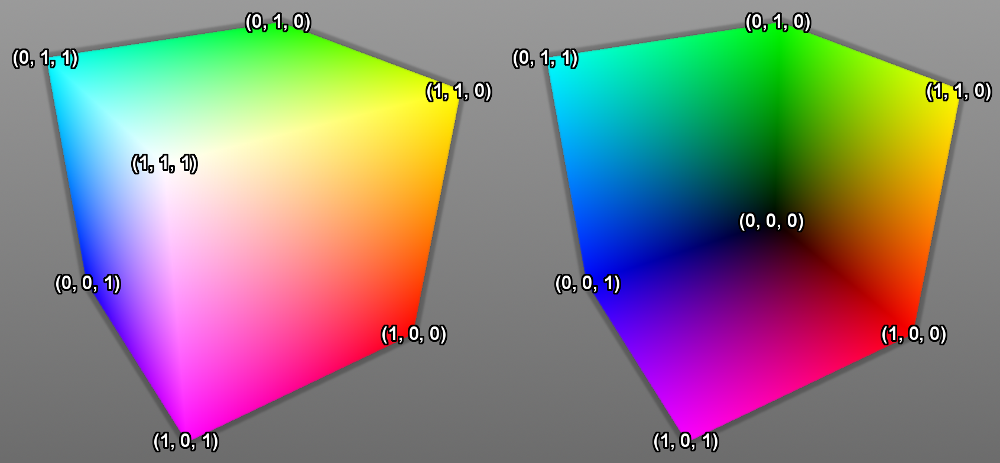
\includegraphics[height=7cm]{color_cubes.png}
\caption{Kairėje pavaizduotas paprastas kubas; dešinėje -- išvirkštinis.}
\label{fig:color_cubes}
\end{figure}

\subsection{Algoritmas}

Pateikiamas algoritmas vienam spindulio skleidimui arba vienam vaizdo gardelės
fragmentui paskaičiuoti. Pristatomame įrankyje šis algoritmas yra vykdomas
darbo autoriaus suprogramuotame GPU fragmentų šeideryje (programa, veikianti
GPU).

\begin{itemize}

\item
Normalaus spalvinio kubo spalvos reikšmė fragmente tampa spindulio kelionės
pradžios taškas

\item
Išvirkštinio spalvinio kubo spalvos reikšmė fragmente tampa spindulio kelionės
pabaigos koordinate

\item
Keliaujame mažu žingsneliu iš pradžios į pabaigos koordinatės poziciją.
Kiekvie-name žingsnelyje kaupiame spalvų ir permatomumo reikšmes pagal šį
ciklą:

\begin{itemize}

\item
Iš duomenų tekstūros nusiskaitome tūrio reikšmę einamoje pozicijoje

\item
Pritaikome transformavimo filtrą

\item
Remdamiesi gradientu, apskaičiuojame apšvietimą

\item
Pritaikome apšveitimo sustiprinimo filtrą

\item
Pritaikome globalų permatomumo filtrą

\end{itemize}

\item
Gautą spindulio skleidimo sankaupos reikšmę išsaugome ir išvedame į ekraną

\end{itemize}

\subsection{GPU panaudojimas}

GPU programuojamumas pasižymi gana dideliais apribojimais. Iš vienos pusės
žvelgiant, tas yra labai nepageidautina. Iš kitos -- tas leidžia GPU
veikiančioms programoms lengvai išskaidyti skaičiavimus į paraleliai
veikiančius GPU procesus.

Pristatomos aplikacijos algoritmas yra būtent toks, koks yra dėl to, kad
norima netrukdyti GPU, kuo galima našiau paskirstyti skaičiavimus. Beveik
visas vizualizacijos generavimas yra paliktas GPU fragmentų procesoriui, nes
pastarasis veiksmas yra izoliuotas nuo aplinkos ir todėl įgalina paskirus
fragmentus apskaičiuoti paraleliai.

Reiktų pabrėžti, kad pačio skaičiavimo išskaidymas nėra įrankio kodo
sudedamoji dalis -- tą atlieka GPU aparatūrinė ir programinė įranga.
Aplikacijoje naudojamas algoritmas tiesiog sudaro sąlygas tam išskaidymui.

\begin{figure}[!ht]
\centering
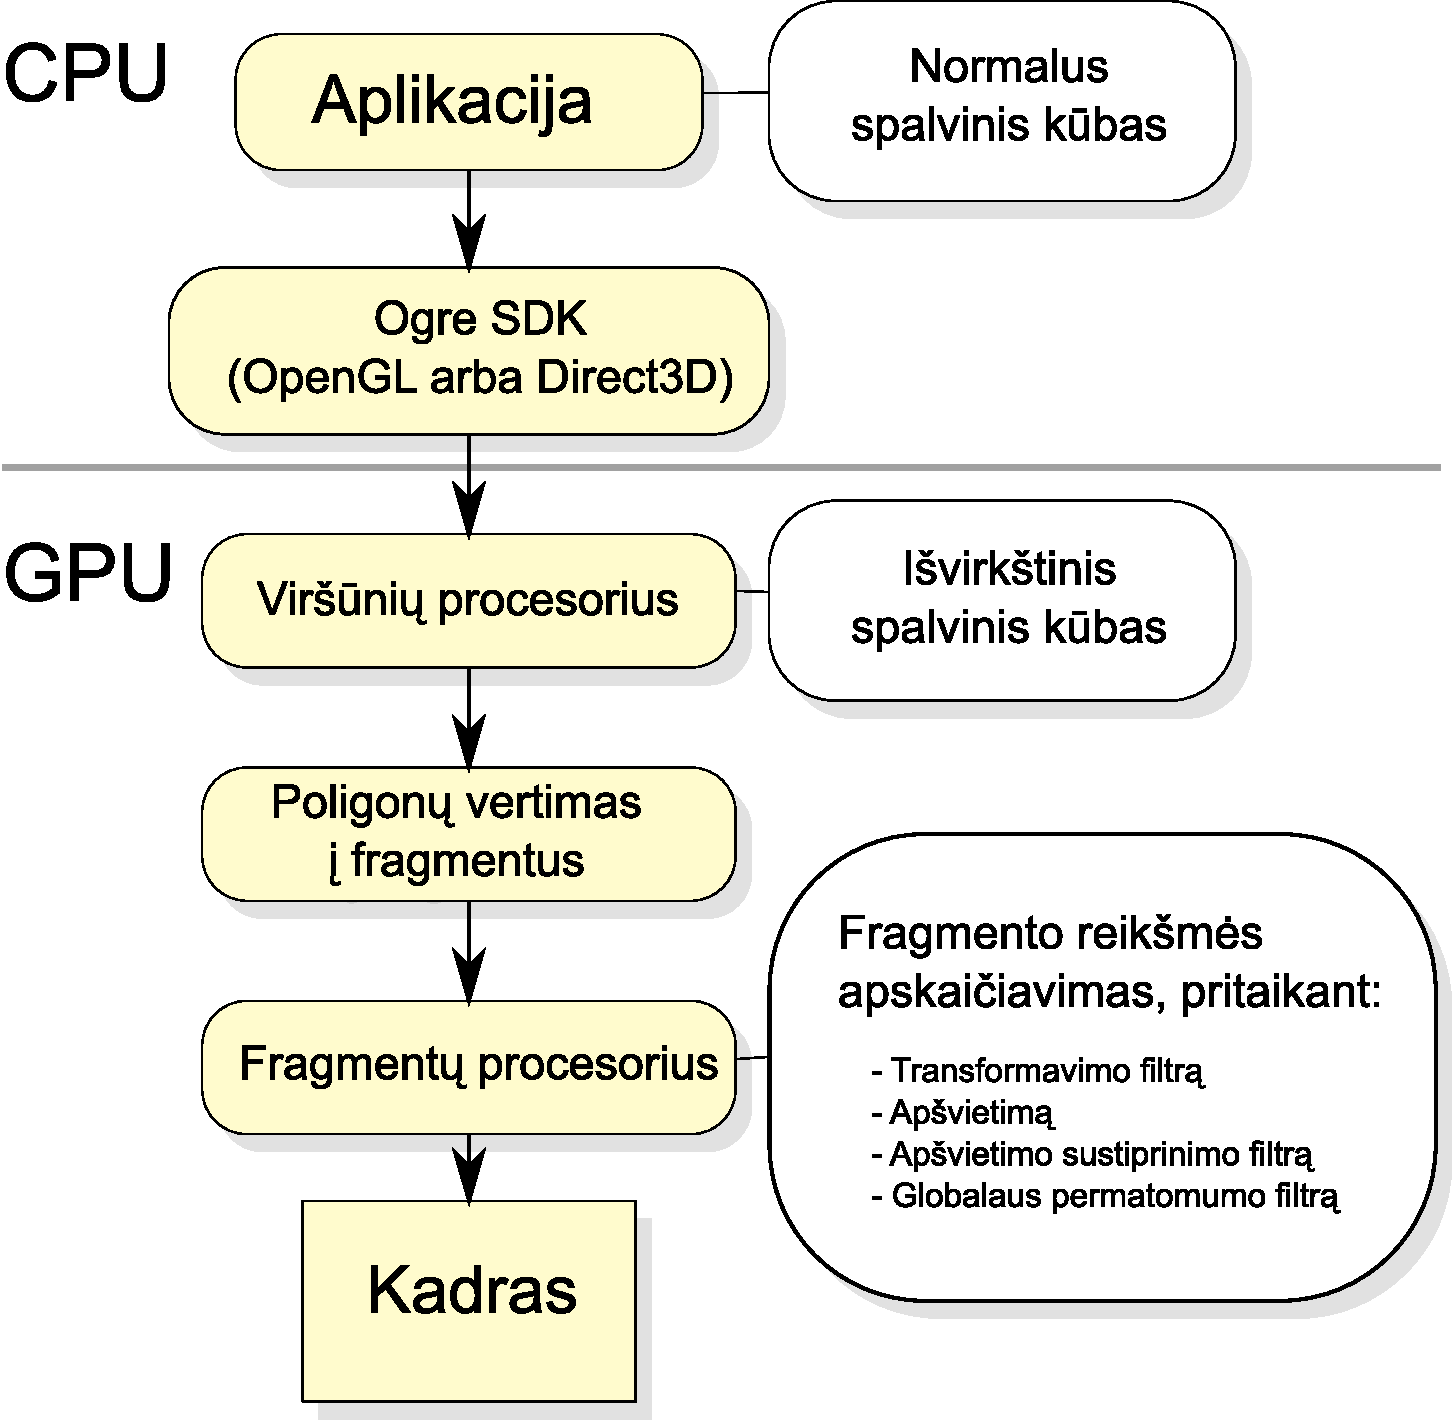
\includegraphics[height=10.0cm]{gpu.pdf}
\caption{GPU panaudojimas įrankyje}
\label{fig:gpu}
\end{figure}

\begin{description}

\item[Aplikacija:] \hfill \\
  Pačioje aplikacijoje apskaičiuojamas normalus spalvinis kubas ir išsaugomas
  tekstūroje, kuri bus nuskaitoma fragmentų procesoriuje. Iš esmės jokio
  skirtumo, kurį kubą pirma skaičiuoti -- galima ir išvirkštinį.

\item[Viršūnių procesorius:] \hfill \\
  Viršūnių procesoriuje apskaičiuojamas išvirkštinis kubas. Tą atlieka
  ganėtinai paprastas skriptas, kuris didžiąją dalį darbo palieka GPU
  aparatūrinei įrangai ir GPU tvarkyklėms.

\item[Fragmentų procesorius:] \hfill \\
  Fragmentų procesoriuje atliekami visi pagrindiniai skaičiavimai, kombinuojant
  abiejų spalvinių kubų ir 3D tekstūroje saugomų vokselių duomenų reikšmes.

\end{description}


\subsection{Transformavimo filtras}

Transformavimo filtras yra funkcija, kurios argumentas yra permatomumo
reikšmė, o rezultatas yra spalva ir nauja permatomumo reikšmė.

$$
F(a') \to \vec{(r, g, b, a)}
$$

\begin{figure}[!ht]
\centering

\includegraphics[height=2.0cm]{transfer.png}
\caption{Permatomumo skalė $0.0 \ldots 1.0$ transformuojama į naują
permatomumo reikšmę, tuo pačiu pridedant spalvos komponentes.}
\label{fig:transfer}
\end{figure}

Transformavimo filtras (Kartais dar vadinamas transformavimo funkcija) buvo
pasiūlytas dar 1988 m., Robert A. Drebin ir kitų veikale \emph{„Volume
Rendering“} \cite{transfer}. Tiesa, tuo metu jie naudojo terminą
klasifikatorius -- „transformavimo funkcija“ terminas buvo pradėtas naudoti
žymiai vėliau. Mano įvesta naujovė yra ta, kad įrankyje transformavimo filtrą
galima keisti realiu laiku. Pokyčiai vizualizacijose vyksta taip pat
realiame laike.

\subsection{Apšvietimo sustiprinimo filtras}

Vizualizuojant tūrinius objektus, turinčius (ar transformavimo funkcijos dėka,
įgaunančius) mažas permatomumo reikšmes, buvo pastebėta, kad detalės pernelyg
susilieja. Tam spręsti siūlomas apšvietimo sustiprinimo filtras.

$$
F(r, g, b, a) = X \cdot D(r, g, b, a) + A(r, g, b, a) + E(r, g, b, a) \to \vec{(r, g, b, a)}
$$

Kur $X$ yra šio filtro parametras; $D$ apšvietimo sklaidos (\emph{diffuse});
$A$ -- apsupties (\emph{ambient}); $E$ -- aplinkos (\emph{environment})
apšvietimo reikšmes skaičiuojančios funkcijos. Pastaba: gradientai, pozicijos
(kameros, šviesos šaltinio, vokselio) aiškumo dėliai yra išmesti iš formulių.

Sustiprinant/susilpninant apšvietimo sklaidos komponentės reikšmę $X$ netgi
iki bendrai 3D apšvietimo logikai prieštaraujančių reikšmių, išryškėja kai
kuri dalis „pasislėpusių“ tūrinio objekto detalių.

\subsection{Globalus permatomumo filtras}

Globalus permatomumo filtras, tai taip pat kuriant įrankį sugalvotas ir šiame
veikale pasiūlytas filtras, kuris savyje kombinuoja tiek slenksčio, tiek
permatomumo reikšmės sustiprinimo/susilpni-nimo filtrus.

$$
F(r, g, b, a) =
\left\{
  \begin{array}{ll}
  (r, g, b, a \cdot X) & \mbox{jeigu $a > X$}\\
  (0, 0, 0, 0) & \mbox{jeigu $a \leq X$}
  \end{array}
\right. \to \vec{(r, g, b, a)}
$$

Kur $X$ yra šio filtro parametras. Pačioje pradžioje, kuriant įrankį, buvo
naudojamas paprastas slenksčio filtras. Tačiau sugeneruotas vaizdas pasižymėjo
grubiais „peršokimais“ slenksčio ribose. Norint to išvengti buvo sugalvotas
filtras, kurio esmė yra siūlymas permatomumą riboti ir slenksčio prieigose.

\subsection{Vokselių trynimo funkcija}

Realaus laiko kompiuterinė grafika skiriasi nuo prieš rodymą sugeneruotos
dviem dalykais: interaktyvia navigacija ir virtualaus pasaulio keitimu.

Pristatomame įrankyje navigacija yra neribojame -- galima judėjimas bet kuria
kryptimi ir kame-ros sukiojimas leidžiamas bet kokiu kampu.

Nenorint palikti virtualaus pasaulio (aprašomos aplikacijos atveju tiesiog
įrankyje rodomo tūri-nio objekto) keitimo funkcijos nuošalyje, yra įdiegtas
grynai demonstracinio pobūdžio vokselių trynimo funkcionalumas.

Tai labai paprastą funkcionalumą turintis įrankio modulis. Jis įgalina
vartotoją šaudyti kiaurai tūrinį objektą. Atlikus šį veiksmą, šūvio kelio
aplinkoje yra pašalinami vokseliai, atliekant aibių skirtumo operaciją.
(Pav. \ref{fig:delete_voxels1} ir \ref{fig:delete_voxels2}).

Šio redagavimo funkcionalumo esmė yra parodyti, kad įrankyje rodomas iš
vokselių sudarytas tūrinis objektas yra vizualizuojamas realiu laiku,
nepritaikant jokių optinių apgaulių ir nesinaudojant jokiais podėliais.
„Šaunant“ per tūrinį objektą, vartotojui iškart yra pateikiamas nauja,
pakitusi vokslelių vizualizacija.

\begin{figure}[t]
\centering
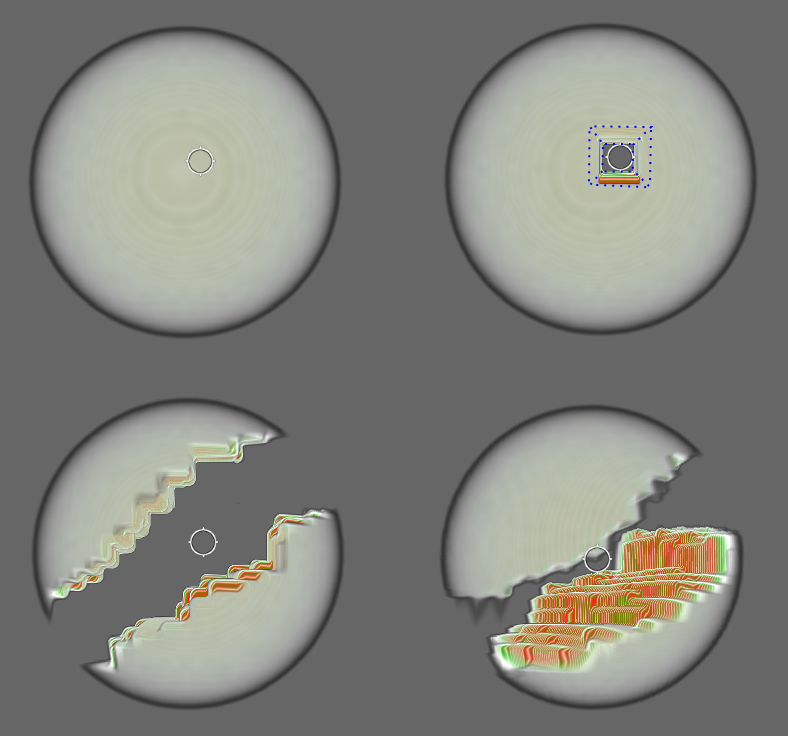
\includegraphics[height=8cm]{delete1.png}
\caption{Vokselių trynimas.}
\label{fig:delete_voxels1}
\end{figure}

\begin{figure}[t]
\centering
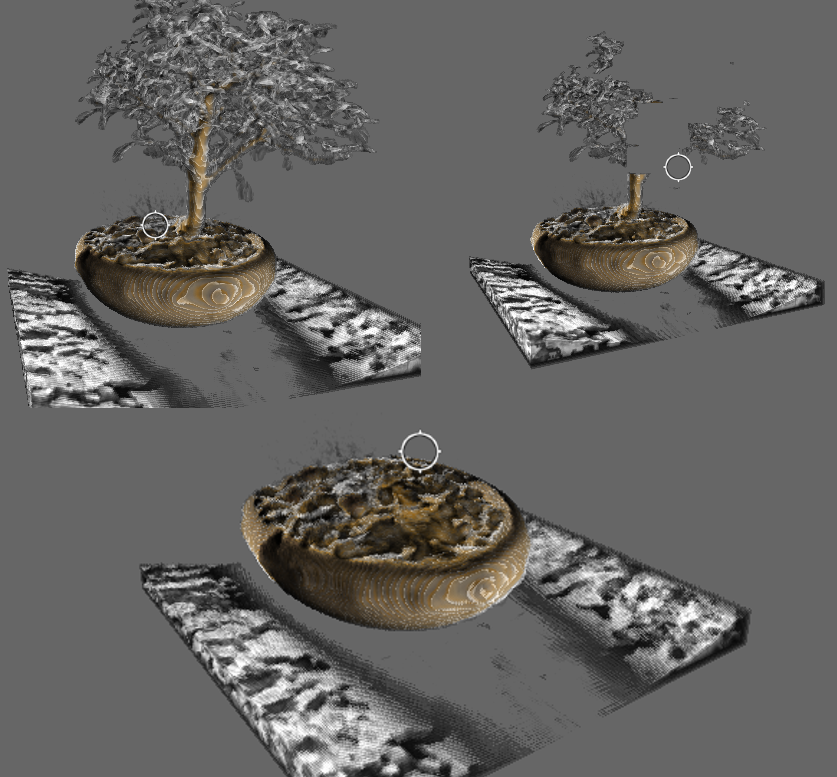
\includegraphics[height=8cm]{delete2.png}
\caption{Vokselių trynimas.}
\label{fig:delete_voxels2}
\end{figure}


\subsection{Naudotos technologijos}

Įrankis kurtas naudojantis šiomis technologijomis: C++ programavimo kalba, Qt
vartotojo sąsajos bibliotekas, OGRE grafinį varikliuką ir Cg šeiderių rašymo
programavimo kalbą.

\subsubsection{OGRE}

OGRE (Object-Oriented Graphics Rendering Engine) yra atviro kodo, lankstus
trimatės kompiuterinės grafikos variklis, sukurtas su C++ programavimo kalba.

Pagrindiniai jo privalumai:

\begin{itemize}

\item
  Atviras kodas

\item
  Palaikoma daugumoje Operacinių sistemų (MS Windows, Linux, Mac OS).

\item
  Palaiko tiek OpenGL ir Direct3D. OGRE variklis leidžia nekreipti dėmesio į
  tai, su kokiomis grafinėmis tvarkyklėmis veikia juo parašyta aplikacija.
  Multiplatformiškumas tampa dvigubas: tiek OS, tiek grafinių tvarkyklių
  požiūriais.

\item
  Lankstumas. Šis variklis netrukdo, jeigu bandoma atlikti kažką egzotiško
  ir/ar neįprasto.

\item
  Bibliotekos moduliai suteikia patogų funkcionalumą daugeliui standartinių
  veik-smų -- susitaupo daug laiko, nes nereikia rašyti pasikartojančio,
  trivialaus kodo.

\end{itemize}

\subsubsection{Qt}

Qt yra multiplatforminis aplikacijų ir vartojo sąsajos kūrimo bibliotekų
rinkinys. Biblioteka skirta grafiniai vartotojo sąsajai sukurti. Ji buvo
naudota langams, bei dialogams sukurti, įvesties (pelė, klaviatūra) veiksmas
apdoroti. Qt pasirinkimą lėmė šios savybės:

\begin{itemize}

\item
  Multiplatforminė biblioteka. Jeigu būtų pasirinkta ne multiplatforminė --
  būtų prarasta visa nauda, gaunama iš to, kad OGRE yra multiplatforminė.

\item
  Atviras kodas.

\item
  Puiki dokumentacija.

\item
  Lengva integracija su OGRE.

\end{itemize}

\subsubsection{Cg}

Cg -- NVidia kompanijos sukurta programavimo kalba, skirta aprašyti GPU
programuojamuo-se procesoriuose vykdomas komandas (\emph{shaders}) (tiek
fragmentų, tiek viršūnių, tiek geometrijos). Išskirtinė tuo, kad kitaip nei
GLSL ar HLSL programavimo kalbos, šioji gali būti kompiliuojama tiek į GLSL,
tiek į HLSL, tiek į asemblerinį išeities kodą. Kaip jau minėta, OGRE įgalina
paleisti pristatomą įrankį tiek OpenGL, tiek Direct3D tvarkykles naudojančiose
OS. Cg pasirinkimas leidžia išlaikyti šį multiplatformiškumą.

\subsection{Apšvietimas}

Vaizdas tėra formos ir apšvietimas. Paprastai kompiuterinėje grafikoje
apšvietimas skaičiuojamas, pasitelkiant paviršių normalias, susietas su
poligonų viršūnėmis. Tuo tarpu įrankyje nėra vizualiai matomų poligonų -- yra
tik vokseliai.

Apšviestiems tūriniams objektams vizualizuoti yra naudojamas gana standartinis
metodas -- kiekvienam vokseliui yra paskaičiuojamas jo permatomumo gradientas.
Įgyvendinant gradientų skaičiavimą buvo remtasi Harvey Ray ir kitų
\cite{gradients} pateiktu apytiksliu gradientų skaičiavimo metodu. Tas
gradientas yra naudojamas kaip normalė standartinėje kompiuterinės grafikos
apšvietimo schemos realizacijoje.

Apytikslio vokselio gradiento, esančio pozicijoje $(i, j, k)$, skaičiavimo
formulė:

$$
G =\Big( \frac{S_{i+1, j, k} - S_{i-1, j, k}}{\Delta x} ,
         \frac{S_{i, j+1, k} - S_{i, j-1, k}}{\Delta y} ,
         \frac{S_{i, j, k+1} - S_{i, j, k-1}}{\Delta z})
$$

Kur $S_{i', j', z'}$ yra vokselio permatomumo (ar tankumo) reikšmė pozicijoje
$(i', j', z')$, o $\Delta a$ -- vokselių atstumas koordinatės $a$ atžvilgiu.

Kadangi toks gradientų skaičiavimas nėra visiškai tikslus, tai ganėtinai mažą
vokselių kiekį turinčių objektų vizualizacijos turi nepageidaujamus
artefaktus. Ši problema įrankyje buvo išspręsta, paliekant galimybę išjungti
apšvietimą. Net ir išjungus apšvietimą, įrankis objektus vizualizuoja
atsižvelgdamas į vokselių nutolimą nuo kameros. Taip vaizdui yra suteikiamas
gilumo pojūtis (Pav. \ref{fig:lighting}).

\begin{figure}
\centering
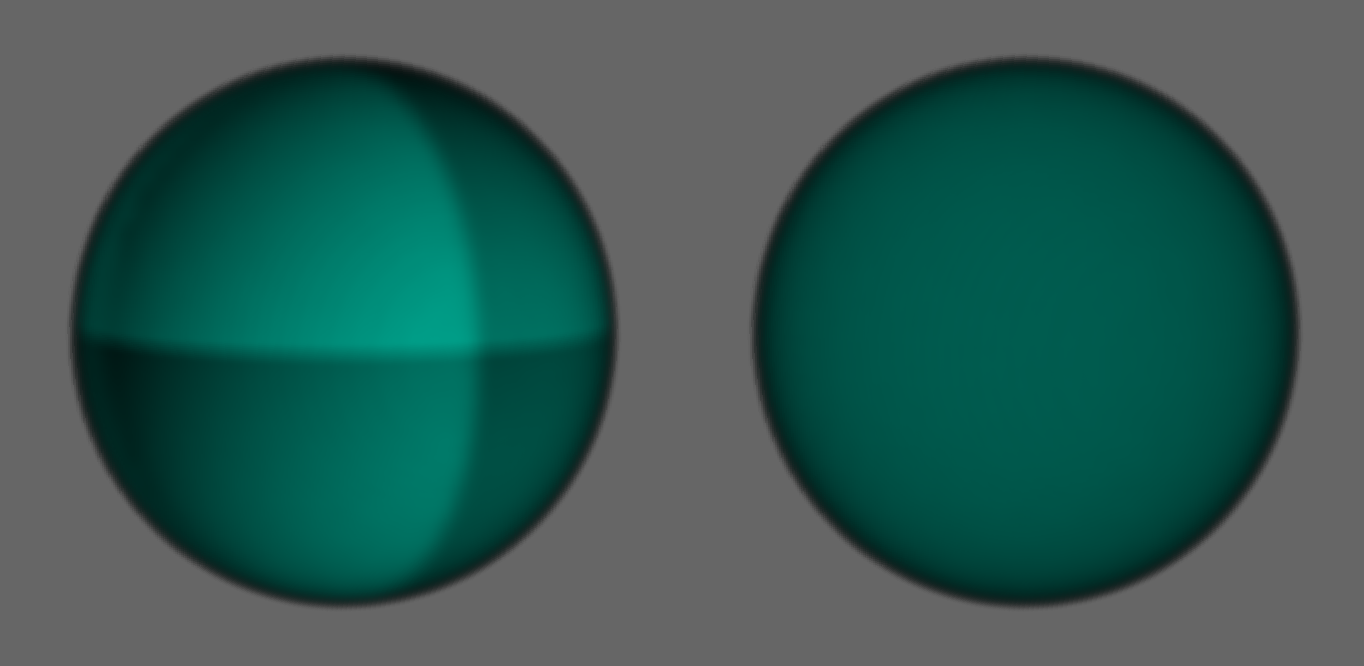
\includegraphics[height=6.0cm]{lighting.png}
\caption{Su apšveitimu ir apšvietimo artefaktais (kairėje); Be apšvietimo
(dešinėje). Pastaba: šviesos šaltinio ir kameros pozicijos specialiai
pasirinktos taip, kad išgauti kuo prastesnį vaizdą.}
\label{fig:lighting}
\end{figure}

\subsection{Spalvoti multi kubai}

Susijusių darbų (\ref{sec:susije_darbai} skyrius) apžvalgoje buvo minėta, kad
daugelis autorių šiuo metu stengiasi pavaizduoti kuo didesnį kiekį vokselių.
Norėdami tą atlikti realiu laiku, jie daro tam tikras prielai-das ir
apribojimus. Tokius kaip:

\begin{itemize}

\item
  Erdvė daugiausia susideda iš tuštumos arba nepermatomų objektų.

\item
  Įvairiose aplikacijose (Pavyzdžiui žaidimuose) vartotojas mato tik nedidelę
  sce-nos dalį.

\item
  Dalinai permatomi objektai retai kada pasitaiko ir dažniausiai yra
  susispietę tam tikrose scenos vietose.

\end{itemize}

Tokios ir panašios prielaidos leidžia jiems atlikti daug optimizacijų.  Tuo
tarpu čia pristatomo įrankio kūrėjas negalėjo sau leisti panašių prielaidų.
Visų pirma dėl to, kad būdama vizualizavimo ir {\bf normavimo} įrankiu,
aplikacija privalo galėti rodyti visą sceną vienu metu. Visų antra, dėl to,
kad yra įgyvendintas interaktyvus transformavimo filtro keitimas, įrankis
negali žinoti, kokias permatomumo reikšmes vokseliai įgis kito kadro metu -- o
reikšmės gali keistis kardinaliai.

Taigi, įrankis priverstas visą sceną laikyti GPU operatyvioje atmintyje.
Norint šiek tiek padidinti kadrų per sekundę skaičių, buvo sugalvota spalvotų
kubų idėją šiek tiek pakoreguoti ir buvo sugalvota spalvotų multi kubų idėją.
Užbėgant už akių, deja, reikia pripažinti, kad pastaroji idėja nedavė jokių
teigiamų rezultatų.

Spalvotų multi kubų idėja ganėtinai paprasta -- vietoje vienos didelės 3D
tekstūros, saugoti scenos tūriniams duomenims, vokseliai yra saugomi $NxNxN$
3D tekstūrose. Buvo tikimasi, kad dėl procesorių gausos GPU, daug mažų
tekstūrų bus našesnis sprendimas, nei viena didelė. Vizualizuojant, buvo
generuojamas vienas išvirkštinis ir $NxNxN$ normalūs spalviniai kubai (Pav.
\ref{fig:multi_color_cubes}).

\begin{figure}[!ht]
\centering
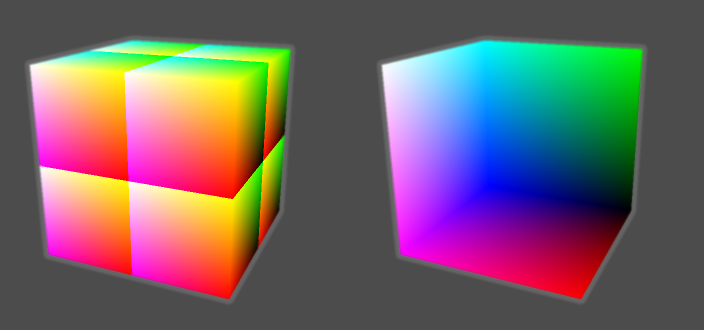
\includegraphics[height=6cm]{multi_color_cubes.png}
\caption{Spalvotų multi kubų idėja}
\label{fig:multi_color_cubes}
\end{figure}

Rezultatai (Lentelė \ref{tab:multi_color_cubes}) nerodo jokių teigiamų pokyčių
\footnote[1]{Naudota techninė įranga: Intel Pentium(R) 4 CPU 3.00GHz; 1 GB
RAM; NVIDIA GeForce 9500 GT (512 MB Ram). Vaizdavimo rezoliucija $846x464$.}
:

\begin{table}[!ht]
\centering
  \begin{tabular}{ | r | r | r | r | }
  \cline{2-4}
  \multicolumn{1}{c|}{} & \multicolumn{3}{|c|}{Scenos padalijimas} \\ \cline{2-4}
  \multicolumn{1}{c|}{} & $1x1x1$ & $2x2x2$ & $4x4x4$ \\ \hline
  262144 vokseliai      &  101.42 &   98.05 &   77.26 \\ \hline
  16777216 vokseliai    &   65.51 &   65.25 &   59.09 \\ \hline
  \end{tabular}
\caption{Spalvotų multi kubų įtaka kadrų per sekundę skaičiui}
\label{tab:multi_color_cubes}
\end{table}

Paaiškėjo, kad (bent jau su testuota aparatūrine įranga) pats suskaidymas neduoda
jokios ap-čiuopiamos naudos -- tiesiog prarandami keli kadrai per sekundę dėl
papildomo darbo skaičiuojant multi kubus.

Tiesa, yra vienas tokio suskaidymo privalumas. Naudojant ją yra įmanoma
pavaizduoti net ir tokias scenas, kurios dėl vokselių skaičiaus netelpa į GPU
atmintį -- ko nebuvo galima atlikti be jos. Reikia pastebėti, kad netelpant
scenai į atmintį, kadrų per sekundę skaičius būna nukritęs į tokias žemumas,
jog to nebegalima vadinti „realiu laiku“.

Taip pat yra dar vienas galimas privalumas. Tikėtina, kad toks ar panašus
priėjimas prie vokselių vizualizavimo duotų naudos, naudojant ne vieną, o
kelis GPU vienu metu. Tačiau tyrimai šia kryptimi nebuvo atlikti dėl to
paprastos priežasties -- autorius neturėjo prieigos prie tokią komplektaciją
turinčios aparatūrinės įrangos.


\section{Rezultatai}

Sukurtas įrankis įgalina realiu laiku iš kartais nevisai gerai ir tiksliai
išsaugotų tūrinių duomenų išgauti akiai daug malonesnius vaizdinius.

Kaip funkcionalumo pavyzdį pateiksiu keturių turinių objektų išvaizdos
apdorojimą, pasiektą šiuo įrankiu.

Pirma, turime tiesioginę vokselių interpretaciją. Vokselių permatomumo
reikšmės tiesiogiai atvaizduojamos skalėje $0.0 \ldots 1.0$ (Pav.
\ref{fig:compare_0}). Tada objektams pritaikomas transformavimo filtras (Pav.
\ref{fig:compare_1}). Objektų išvaizda dar šiek tiek pakoreguojama globaliu
permatomumo filtru (Pav. \ref{fig:compare_2}). Galiausiai pritaikomas
apšvietimo sustiprinimo filtras ir gaunamas galutinis vaizdas (Pav.
\ref{fig:compare_3}).

Kaip jau minėta, įrankis nėra skirtas dideliam kiekiui, ar dideliam
vaizdavimo greičiui pasiekti -- tai kitų temų sritis. Tačiau, realaus laiko
savoka įpareigoja pateikti kadrų per sekundę rezultatus\footnote[1]{Naudota techninė įranga: Intel Pentium(R) 4 CPU 3.00GHz; 1 GB
RAM; NVIDIA GeForce 9500 GT (512 MB Ram). Vaizdavimo rezoliucija $846x464$.}

(Lentelė \ref{tab:fps}).

\begin{table}[!ht]
\centering
  \begin{tabular}{ | r | r | r | r | }
  \cline{1-4}
  Scenos padalijimas    &     $49x49x49$ &    $64x64x64$ & $98x34x34$   \\ \hline
  Kadrai per sekundę    &          96.01 &         93.54 &      90.24   \\ \hline
  Scenos padalijimas    &  $256x256x128$ & $256x256x256$ & $301x324x56$ \\ \hline
  Kadrai per sekundę    &          59.21 &         59.24 &        50.28 \\ \hline
  \end{tabular}
\caption{Kadrai per sekundę (vidurkis), vaizduojant įvairių dydžių tūrinius objektus. }
\label{tab:fps}
\end{table}

\begin{figure}[b]
\centering
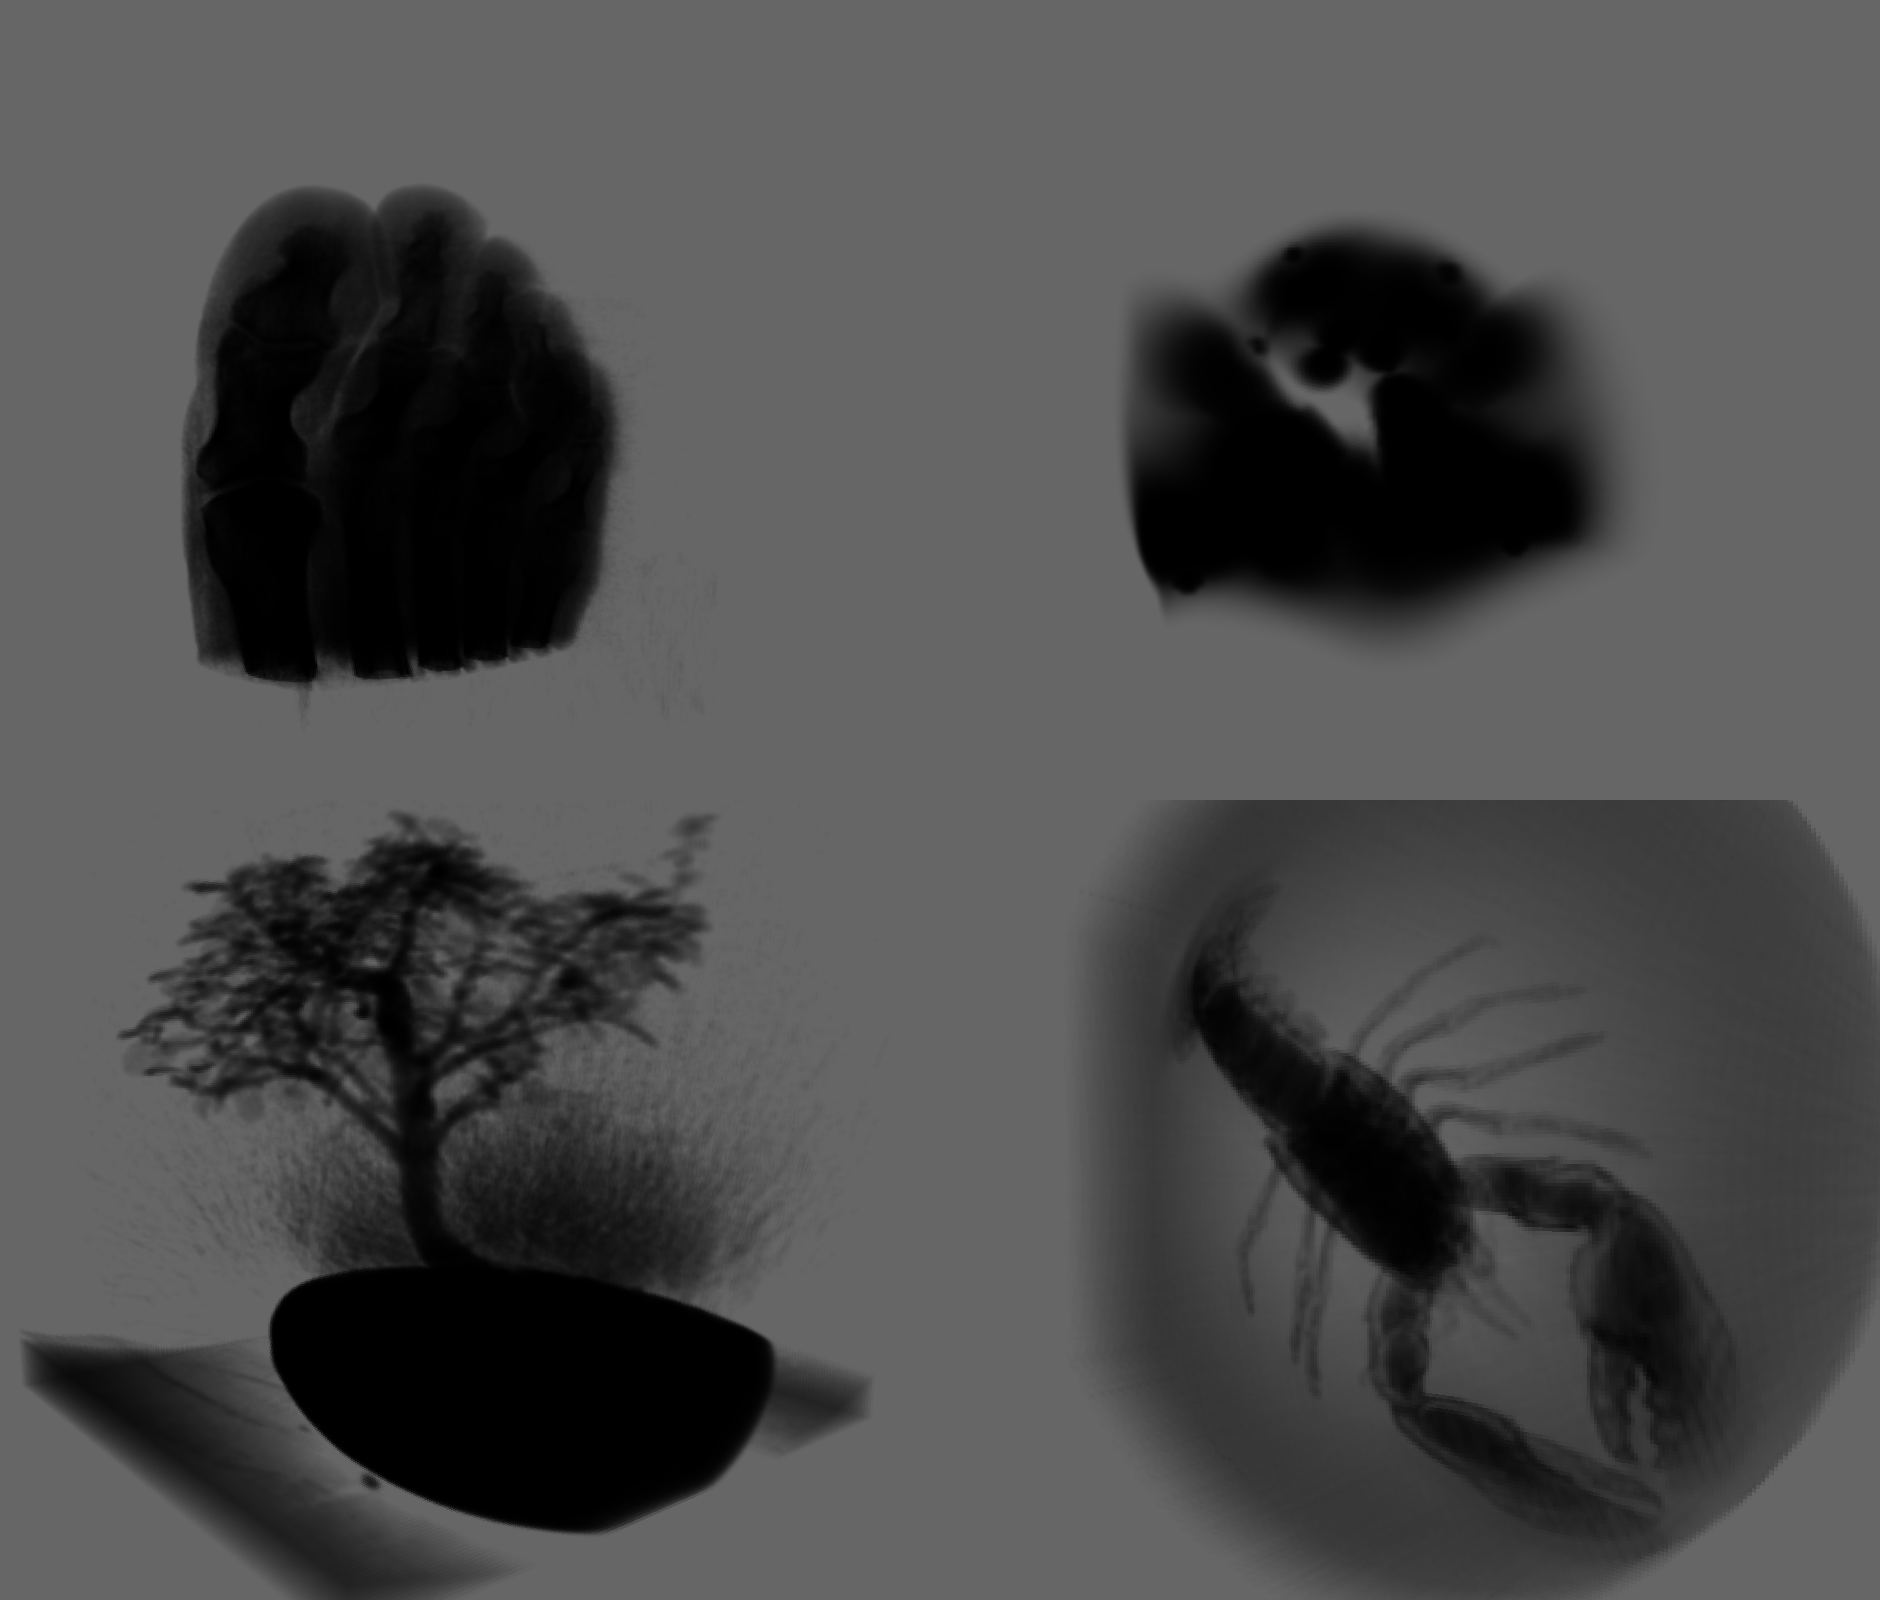
\includegraphics[height=11.5cm]{compare_0.png}
\caption{Pradinės tūrinių objektų vizualizacijos.}
\label{fig:compare_0}
\end{figure}

\begin{figure}[b]
\centering
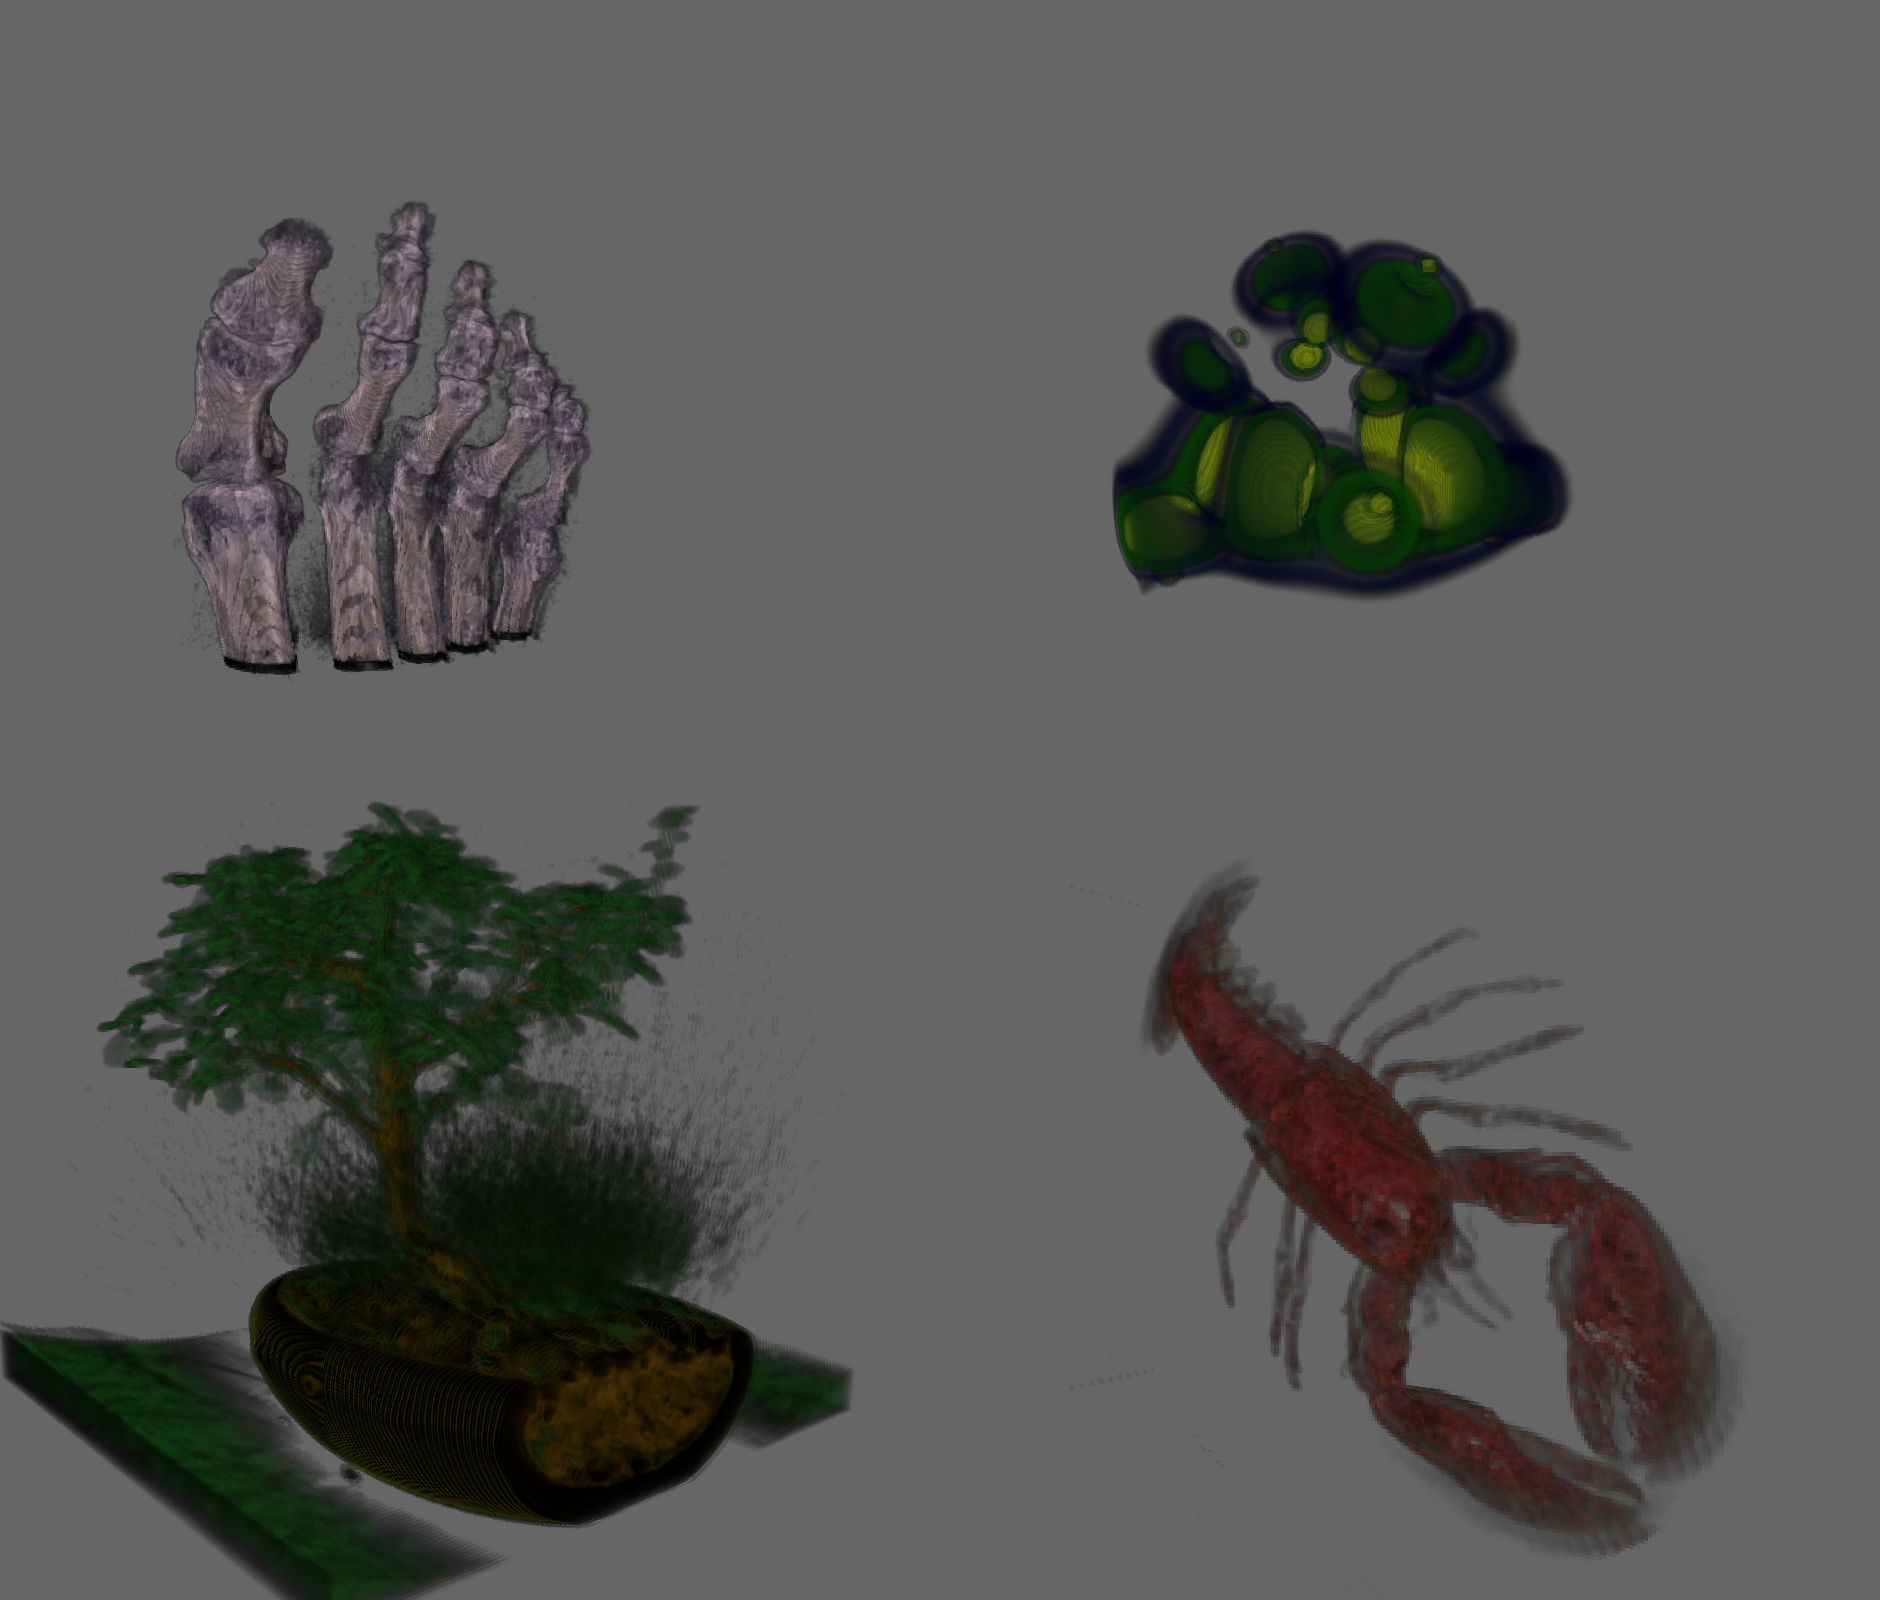
\includegraphics[height=11.5cm]{compare_1.png}
\caption{Transformavimo filtras.}
\label{fig:compare_1}
\end{figure}

\begin{figure}[b]
\centering
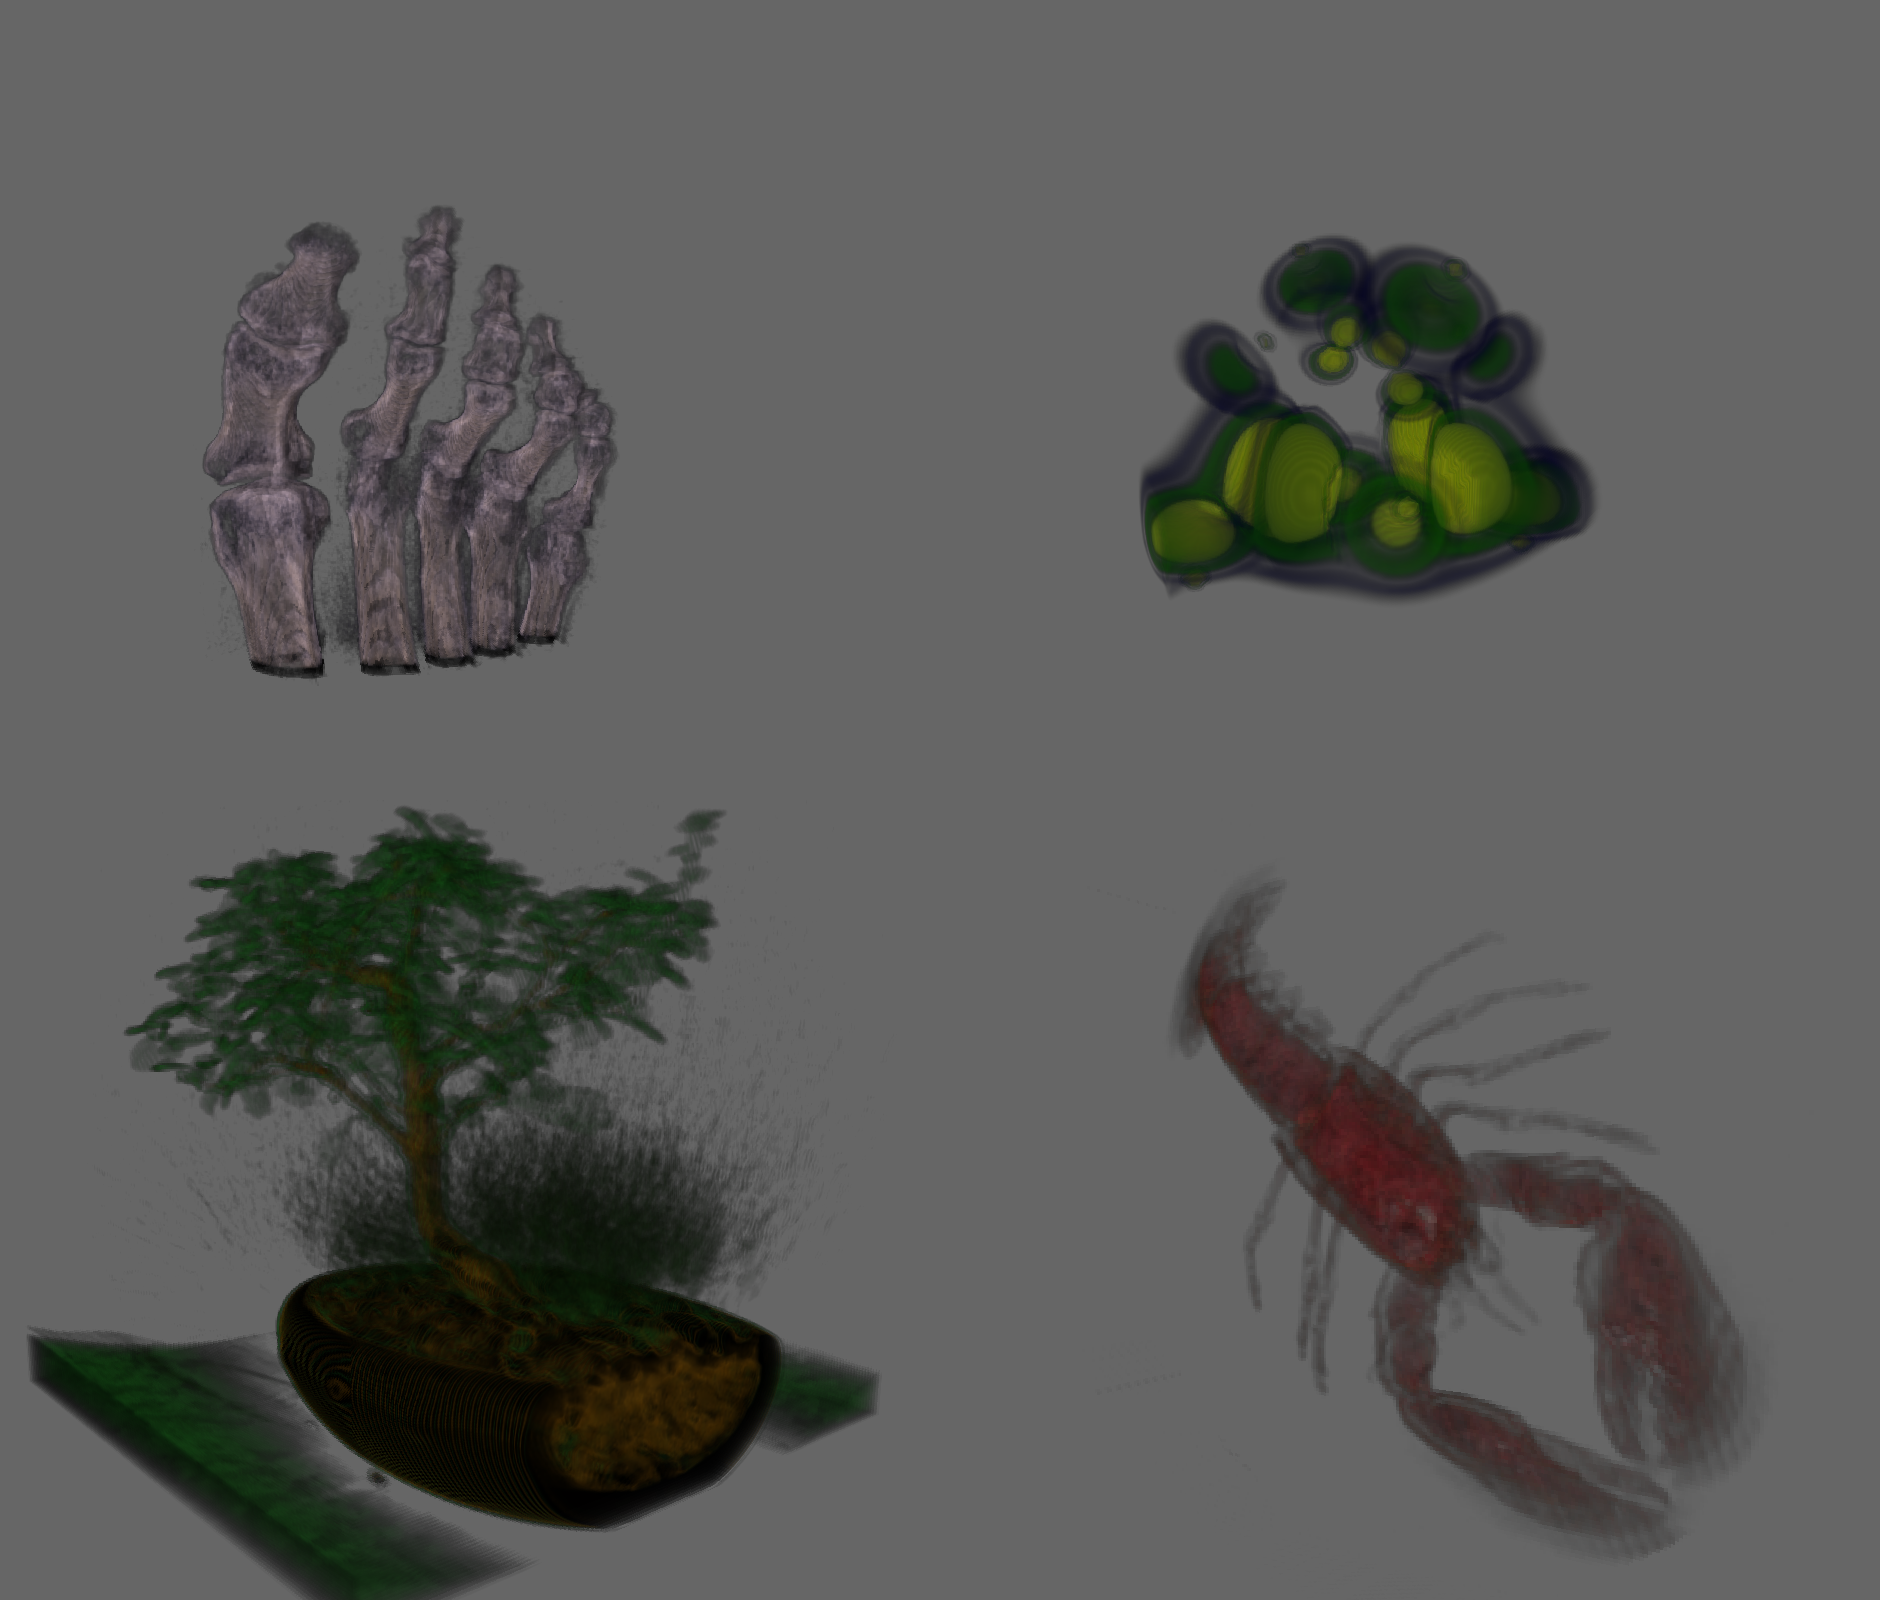
\includegraphics[height=11.5cm]{compare_2.png}
\caption{Globalaus permatomumo filtras.}
\label{fig:compare_2}
\end{figure}

\begin{figure}[b]
\centering
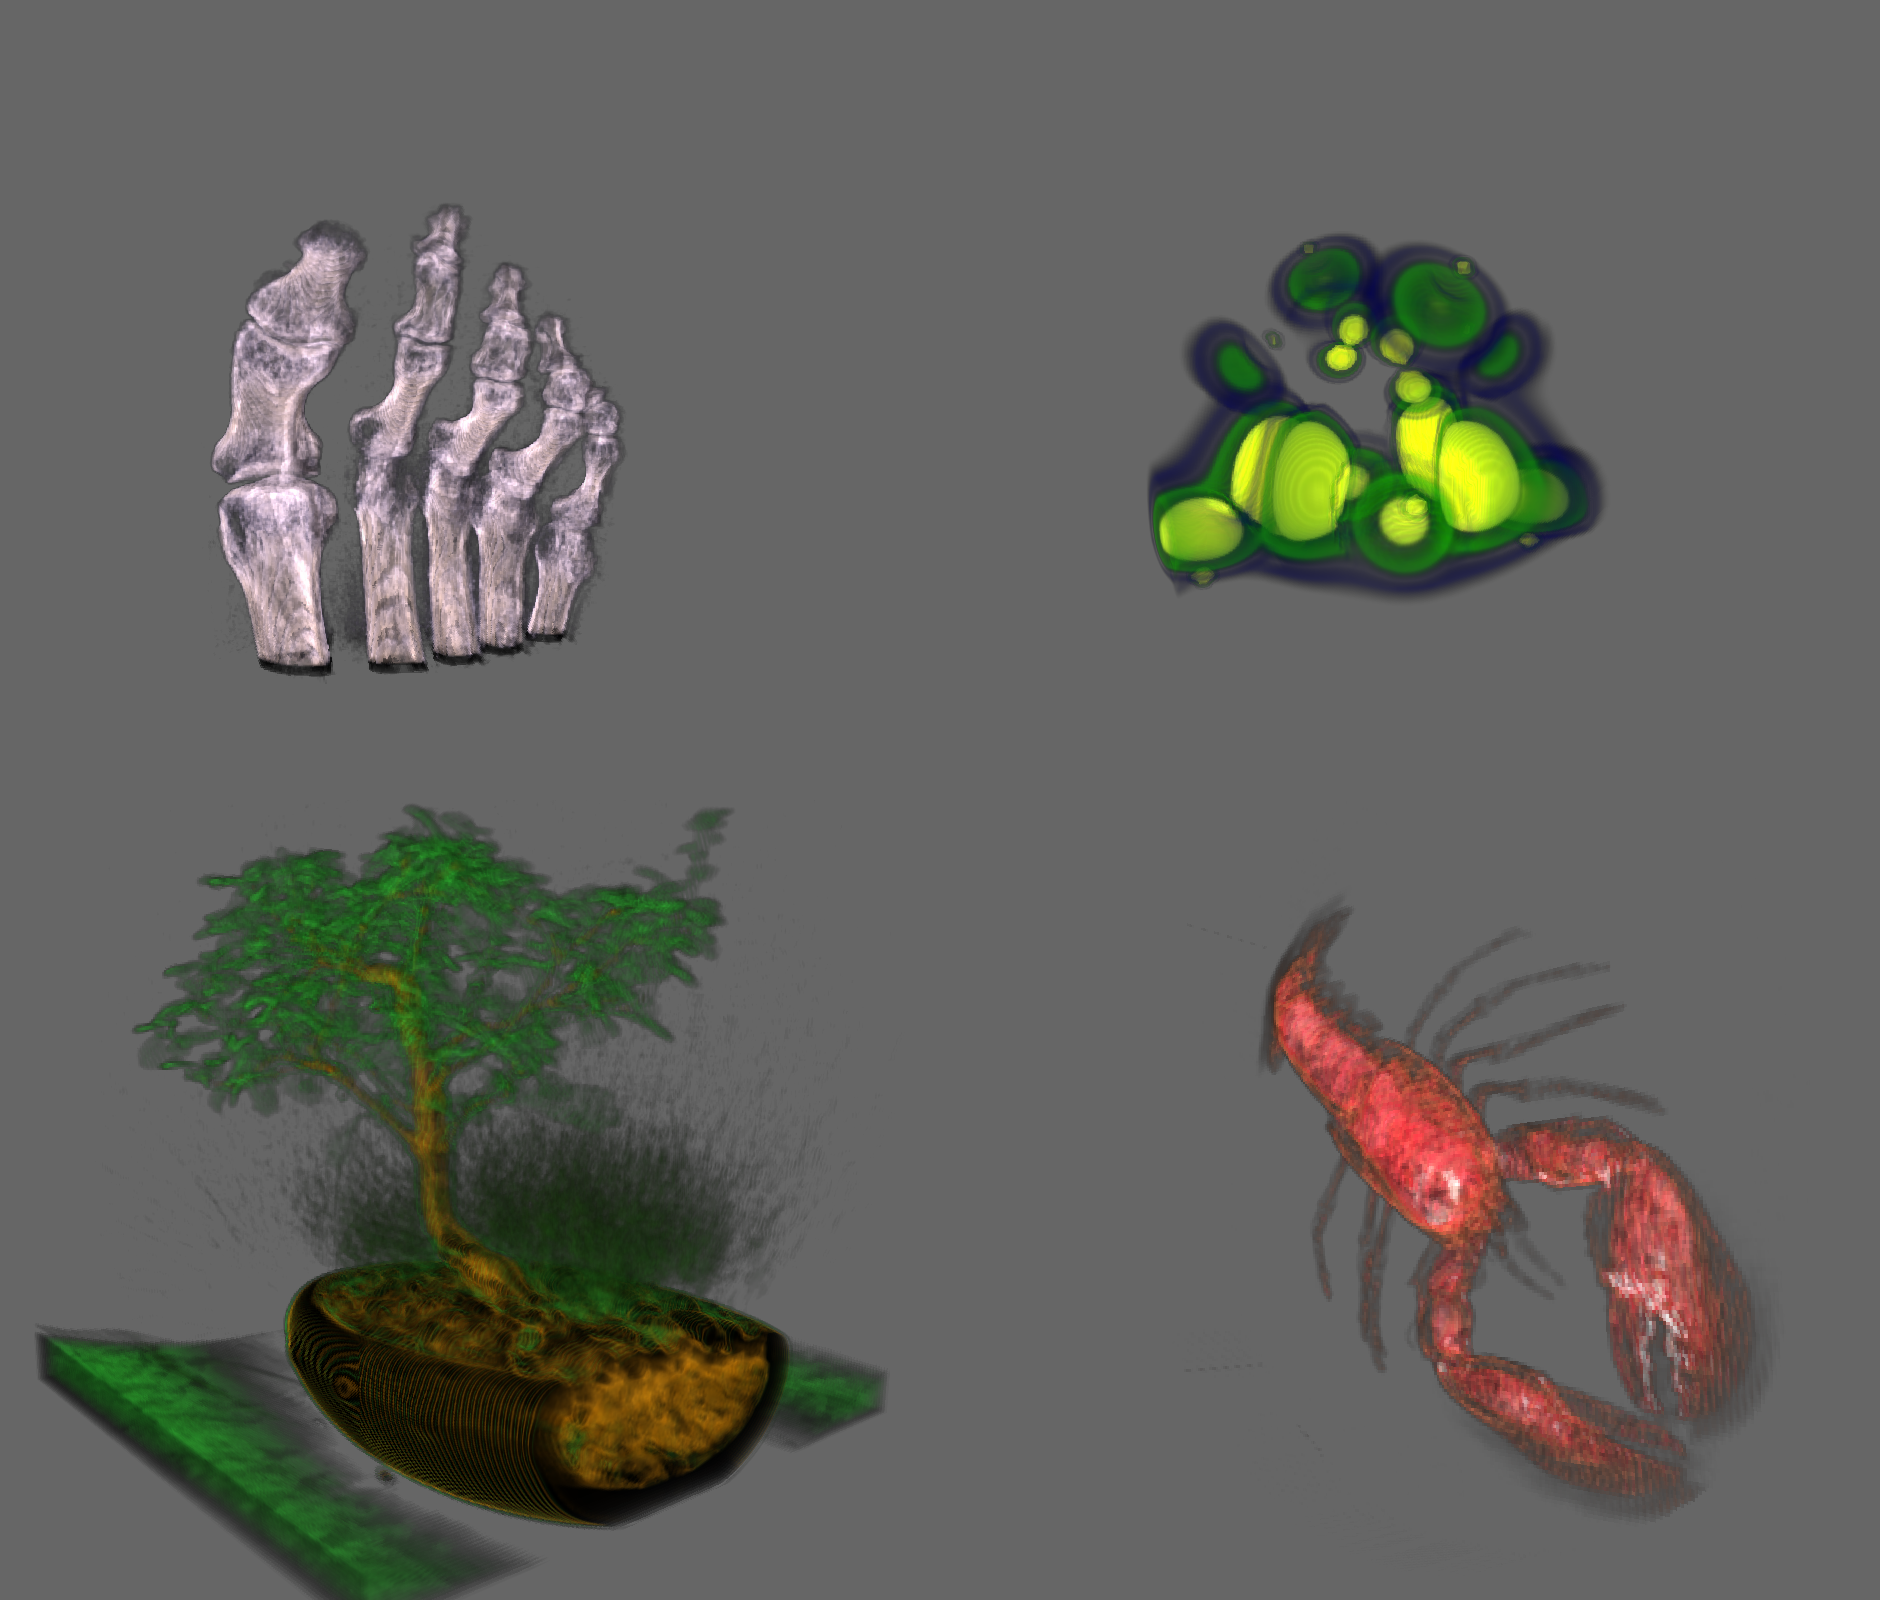
\includegraphics[height=11.5cm]{compare_3.png}
\caption{Apšvietimo sustiprinimo filtras.}
\label{fig:compare_3}
\end{figure}


\section{Išvados}

Šiame darbe buvo pristatytas vokselių vizualizavimo ir normavimo įrankis,
prieš tai pristatant pačius vokselius, jų vizualizavimo idėjas ir panaudojimą
įvairiose srityse.

Bekuriant įrankį buvo sukurtas realaus laiko transformavimo filtro modulis,
leidžiantis greitai ir paprastai pritaikyti vokselių permatomumo reikšmes
vizualizuojamam vaizdui. Taip pat buvo sugalvoti du nauji filtrai.

Pirmas, globalaus permatomumo filtras leidžia pritaikyti permatomumo slenksčio
modifikaciją, išvengiant grubaus peršokimo slenksčio prieigose, atsirasdavusio
naudojant tik slenksčio filtą. Re-zultatas -- subtilus vaizdo pagerėjimas,
geriausiai matomas, prieš tai pritaikius kontrastingą transformavimo filtrą.

Antras, apšvietimo sustiprinimo filtras leidžia išryškinti dėl permatomumo
susiliejančias tūrinio objekto detales. Pritaikius filtrą generuojamos
vizualizacijos pastebimai įgauna kokybiškesnį ir akiai malonesnį vaizdą.

Darbe taip pat pateikiama spalvotų kubų idėja, kuri nebuvo iki galo ištyrinėta
dėl tinkamos aparatūrinės įrangos stokos.


\clearpage
\phantomsection
\cleardoublepage
\addcontentsline{toc}{section}{\literature}
\begin{thebibliography}{MMM99}

\bibitem[LOR87]{bib:marching-cubes}
  {\bf William E. Lorensen, Harvey E. Cline}\\
  {\em Marching Cubes: A high resolution 3D surface construction algorithm.}\\
  In: Computer Graphics, Vol. 21, Nr. 4, 1987.

\bibitem[CRA09]{gig2009}
  {\bf Cyril Crassin, Fabrice Neyret, Sylvain Lefebvre, Elmar Eisemann}\\
  {\em GigaVoxels: Ray-Guided Streaming for Efficient and Detailed Voxel
  Rendering.}\\
  ACM SIGGRAPH Symposium on Interactive 3D Graphics and Games (I3D), 2009.

\bibitem[CRA08]{gig2008}
  {\bf Cyril Crassin, Fabrice Neyret, Sylvain Lefebvre}\\
  {\em Interactive GigaVoxels Technical Report}\\
  INRIA Technical Report, 2008.

\bibitem[GOB08]{other}
  {\bf Enrico Gobbetti, Fabio Marton, Jose Antonio Iglesias Guitian}\\
  {\em A single-pass GPU ray casting framework for interactive out-of-core
  rendering of massive volumetric datasets.}\\
  The Visual Computer: International Journal of Computer Graphics, 2008.

\bibitem[KRÜ03]{raycast}
  {\bf Jens Krüger ir Rüdiger Westermann}\\
  {\em Acceleration Techniques for GPU-based Volume Rendering.}\\
  Computer Graphics and Visualization Group, Technical University Munich, 2003.

\bibitem[RAY99]{gradients}
  {\bf Harvey Ray, Hanspeter Pfister, Deborah Silver, Todd A. Cook}\\
  {\em Ray Casting Architectures for Volume Visualization.}\\
  MITSUBISHI ELECTRIC RESEARCH LABORATORIES, 1999.

\bibitem[DRE88]{transfer}
  {\bf Robert A. Drebin, Loren Carpenter ir Pat Hanrahan}\\
  {\em Volume Rendering.}\\
  Computer Graphics, Volume 22, Number 4, August 1988.

\bibitem[LEV87]{first}
  {\bf Marc Levoy}\\
  {\em Display of Surfaces from Volume Data.}\\
  Computer Science Department University of North Carolina Chapel Hill, NC 27514. 1987

\end{thebibliography}


\end{document}

